%------------------------------------------------------------------------------
%	REQUIRED PACKAGES AND  CONFIGURATIONS
%------------------------------------------------------------------------------
%%%
%%%   DRACULA THEME
%%%
%\usepackage{/home/lorenzo/latex_dracula/draculatheme}
\documentclass{article}
%PACKAGES FOR TITLES
\usepackage{titlesec}
\usepackage{color}
\usepackage{tabularx}
\usepackage{multirow}
\usepackage[table]{xcolor}
\usepackage{titling}
\usepackage{nomencl}
\usepackage{biblatex} %Imports biblatex package
\addbibresource{bibliography.bib} %Import the bibliography file

% PACKAGES FOR LANGUAGE AND FONT
\usepackage[utf8]{inputenc}
\usepackage[english]{babel}
\usepackage[T1]{fontenc} % Font encoding

%TIKZ 
\usepackage{tikz}

% TIKZ PACKAGES
\usetikzlibrary{calc,patterns,angles,quotes}
\usepackage{pgfplots}
\pgfplotsset{compat = newest,width=6cm}
\usetikzlibrary{patterns.meta,decorations.pathmorphing}

% PACKAGES FOR IMAGES
\usepackage{graphicx}
\usepackage{float}
\usepackage{wrapfig}
\usepackage{import}
\usepackage{cancel}
\usepackage{xifthen}
\usepackage{pdfpages}
\usepackage{xcolor}
\usepackage{transparent}

\usepackage[acronym]{glossaries}

\makeglossaries

\newcommand{\incfig}[2]{%
    \ifthenelse{\isempty{#2}}{%
        \def\svgwidth{.75\columnwidth}
    }{%
        \def\svgwidth{#2\columnwidth}
    }%
    \import{./figures/}{#1.pdf_tex}
}

% PACKAGES FOR MATH
\usepackage{amsmath}
%\usepackage{siunitx}
% PACKAGES FOR REFERENCES & BIBLIOGRAPHY
\usepackage[colorlinks=true,linkcolor=black!40!black,anchorcolor=black,citecolor=black,filecolor=black,menucolor=black,runcolor=black,urlcolor=black]{hyperref} % Adds clickable links at references
\usepackage[english]{cleveref}
\pdfsuppresswarningpagegroup=1
%-------------------------------------------------------------------------
%	NEW COMMANDS DEFINED
%-------------------------------------------------------------------------
% EXAMPLES OF NEW COMMANDS -> here you see how to define new commands
\newcommand{\e}[1]{\times{} 10^{#1}}  % Powers of 10 notation
\newcommand{\mathbbm}[1]{\text{\usefont{U}{bbm}{m}{n}#1}} % From mathbbm.sty
\newcommand{\pdev}[2]{\frac{\partial#1}{\partial#2}}
\newcommand{\question}[1]{\colorbox{yellow}{#1}}
\newcommand{\integral}[4]{\int_{#1}^{#2} #3 \,\,\diff{} #4}
\newcommand{\dermat}[2]{\frac{\operatorname{D}#1}{\operatorname{D}#2}}
\newcommand{\abs}[1]{|#1|}
\newcommand{\person}[1]{\textsf{#1}}
\newcommand{\R}{\mathbbm{R}}
\newcommand{\costante}{\operatorname{cost}}
%\newcommand{\ln}{\operatorname{ln}}
\newcommand{\diff}{\operatorname{d}}
\newcommand{\vvline}{||}
\newcommand{\prodc}{\displaystyle\prod}
\newcommand{\parallelsum}{\mathbin{/\mkern-5mu/}}
\newcommand{\twomini}[2]{\begin{figure}[H]
                \centering
		\begin{minipage}{.5\linewidth}
			#1
		\end{minipage}
		\begin{minipage}{.5\linewidth}
			#2
		\end{minipage}
\end{figure}}
\newcommand{\twominisw}[4]{\begin{figure}[H]
                \centering
		\begin{minipage}{#3\linewidth}
			#1
		\end{minipage}
		\begin{minipage}{#4\linewidth}
			#2
		\end{minipage}
              \end{figure}}
            \newcommand{\threemini}[3]{\begin{figure}[H]
                \centering
                \begin{minipage}{.3\linewidth}
			#1
		\end{minipage}
		\begin{minipage}{.3\linewidth}
			#2
		\end{minipage}
		\begin{minipage}{.3\linewidth}
			#3
		\end{minipage}
\end{figure}}
%----------------------------------------------------------------------------
%	COLOURS 
%----------------------------------------------------------------------------
\definecolor{darkorange}{RGB}{229, 112, 0}
\definecolor{darkpurple}{RGB}{119, 25, 170}
\usepackage{xifthen}
\makeatother
\def\@lecture{}%
\newcommand{\lecture}[3]{
    \ifthenelse{\isempty{#3}}{%
        \def\@lecture{Lezione #1}%
    }{%
        \def\@lecture{Lezione #1: #3}%
    }%
    \subsection*{\@lecture}
    \marginpar{\small\textsf{\mbox{#2}}}
}

\usepackage{fancyhdr}
%\pagestyle{fancy}
\fancypagestyle{plain}{%
\fancyhf{} % cancella tutti i campi di intestazione e pi\‘e di pagina
\fancyfoot[C]{\bfseries \thepage} % tranne il centro
\renewcommand{\headrulewidth}{0pt}
\renewcommand{\footrulewidth}{0pt}}


% LE: left even
% RO: right odd
% CE, CO: center even, center odd
% My name for when I print my lecture notes to use for an open book exam.
% \fancyhead[LE,RO]{Lorenzo Pasqui}

% \fancyhead[RO,LE]{\@lecture} % Right odd,  Left even

% Right even, Left odd
%\fancyhead[R]{qualcosa}% TODO Aggiungi nomi 

% \fancyfoot[RO,LE]{}  % Right odd,  Left even
% \fancyfoot[RE,LO]{}          % Right even, Left odd
%\fancyfoot[C]{\thepage}     % Center

\makeatother

% redefinition of \maketitle with a logo ==============  
\makeatletter
\newcommand{\logo}[1]{\gdef\@logo{#1}}%
% \def\maketitle{
% \begin{center}
% \setlength\baselineskip{8ex}
% \setlength\parskip{4em plus 1fil minus 3em}
% \includegraphics[width=\textwidth,
% height=.6\textwidth,keepaspectratio]{\@logo}\par
% {\Huge\sffamily\bfseries \@title}\par
% {\Large\scshape \@author}\par
% \end{center}
% \newpage}
% \makeatother
%  end of redefinition  ===============================  \pdfsuppresswarningpagegroup=1
\logo{PoliLogo.jpg}
\author{Palusci Luca
	\\ 
	10730959 
\and
	 Pasqui Lorenzo 
	\\
        10703226
	\\
 \and
	Stellacci Andrea 
	\\ 
	10724258 
	\\
 \and
	Sharmoukh Carlo 
	\\ 
	Codice persona:
 }
 
	\date{11 Agosto 2024}
\newcommand{\myimage}{
\includegraphics[width=0.2\textwidth]{relazione_latex/figures/PoliLogo.jpg}}
\newcommand{\mytitlepage}[1]{%
   \begin{center}
       \myimage
       \vspace{1cm} % Aggiungi spazio tra l'immagine e il titolo
       \LARGE #1
   \end{center}
}

%%% Local Variables:
%%% mode: latex
%%% TeX-master: f
%%% End:

\usepackage[a4paper,top=2cm,bottom=2cm,left=2cm,right=2cm]{geometry}
% dove sono le immagini'
\graphicspath{ {./figures/} }
\pagenumbering{Roman}

% ACRONIMI
% \newacronym{label}{acronimo}{acronimo esteso}
\newacronym{sts}{STS}{Space Transportation System}
\newacronym{iss}{ISS}{International Space Station}
\newacronym{nasa}{NASA}{National Aeronautics and Space Administration}
\newacronym{ssme}{SSME}{Space Shuttle Main Engine}
\newacronym{srb}{SRB}{Solid Rocket Boosters}
\newacronym{lh2}{$LH_2$}{Liquid Hydrogen}
\newacronym{lox}{$LO_2$}{Liquid Oxygen}
\newacronym{lch4}{$LCH_4$}{Liquid Methane}
\newacronym{lptp}{LPTP}{Low Pressure Turbopump}
\newacronym{hptp}{HPTP}{High Pressure Turbopump}
\newacronym{et}{ET}{External Tank}
\newacronym{slwt}{SLWT}{Super Light Weight}
\newacronym{lwt}{LWT}{Light Weight}
\newacronym{hpotp}{HPOTP}{High-Pressure Oxygen Turbopump}
\newacronym{lpotp}{LPOTP}{Low-Pressure Oxygen Turbopump}
\newacronym{hpftp}{HPFTP}{High-Pressure Fuel Turbopump}
\newacronym{lpftp}{LPFTP}{Low-Pressure Fuel Turbopump}
\newacronym{cea}{CEA}{Chemical Equilibrium with Applications}
\makenomenclature
\title{
\begin{center}
\normalsize Aerospace Propulsion\\ \small Final Report\\ \Large \textbf{Space Shuttle Main Engine: fuel and tank analysis}
\end{center}
}
\pretitle{%
	\begin{center}
		\includegraphics[scale=0.1]{Polilogo.jpg}
	\end{center}
 }
        
%\title{Politecnico di Milano \\ \large Aerospace propulsion final report\\ \Large Space Shuttle Main Engine: fuel and tank analysis}

\begin{document}
\maketitle
\newpage
    \section*{Abstract}
     This project focuses on the redesign of the \acrfull{ssme}, aiming to analyze and optimize the engine's performance first using its original propellant — \acrfull{lox} and \acrfull{lh2} — and subsequently with \acrfull{lch4} replacing hydrogen.
     The sizing process is driven by key parameters of the thermodynamic cycle, especially system operating pressures, and includes a detailed assessment of the main components, such as the combustion chamber, nozzles, turbopumps, and the external tank.

   The combustion chamber pressure for the methane redesign was estimated based on the Raptor engine developed by SpaceX, which also utilizes liquid methane with \acrlong{lox}.
   This estimation allowed for a realistic and practical approach to the redesign process.
   Importantly, the project emphasizes not just the engine's performance but also the critical aspect of component sizing, particularly in adapting the external tank to accommodate the different oxidizer-to-fuel (O/F) ratios — 6.032 for \acrshort{lh2} and 3 for methane.

   In the initial phase, a comprehensive review of the engine's performance using the original propellant is conducted, focusing on combustion chamber pressure and specific impulse ($I_{sp}$) to establish a baseline.
   The subsequent redesign phase, incorporating liquid methane, involves adapting key components, including nozzle geometry, expansion ratio, and turbopump characteristics, to maintain optimal efficiency and performance.

   The project demonstrates that liquid methane is a viable alternative, offering benefits in propellant density, chemical stability, and thermal management. However, the primary focus was on the precise sizing of components, particularly ensuring the external tank's capacity and configuration align with the new O/F ratio, while maintaining high combustion chamber pressures to optimize the engine's overall efficiency.
   \newpage
\tableofcontents
    \newpage
% LIST OF FIGURES
\printnomenclature 
    \newpage
    \printglossary[type=\acronymtype]
\newpage
\listoffigures
% LIST OF TABLES
\listoftables

    \clearpage
    \pagenumbering{arabic}
% --- SCRIVERE QUI ---
    \section{Introduction} \label{intro}
 % Space exploration represents one of the most fascinating and complex frontiers of contemporary science and technology. 
%	At the heart of this field is the \acrfull{sts}, commonly known as the Space Shuttle launch system, which played a fundamental role in the development of human capabilities to explore and utilize space.
\begin{wrapfigure}{r}{0.2\textwidth} 
    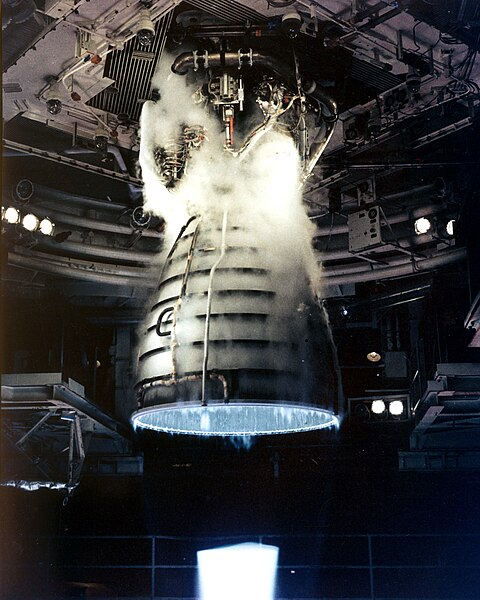
\includegraphics[width=0.2\textwidth]{ssmeTestFiring.jpg}
    \caption{a close-up view of a Space Shuttle Main Engine during a test firing}
    \label{fig:ssmetestfiring}
 %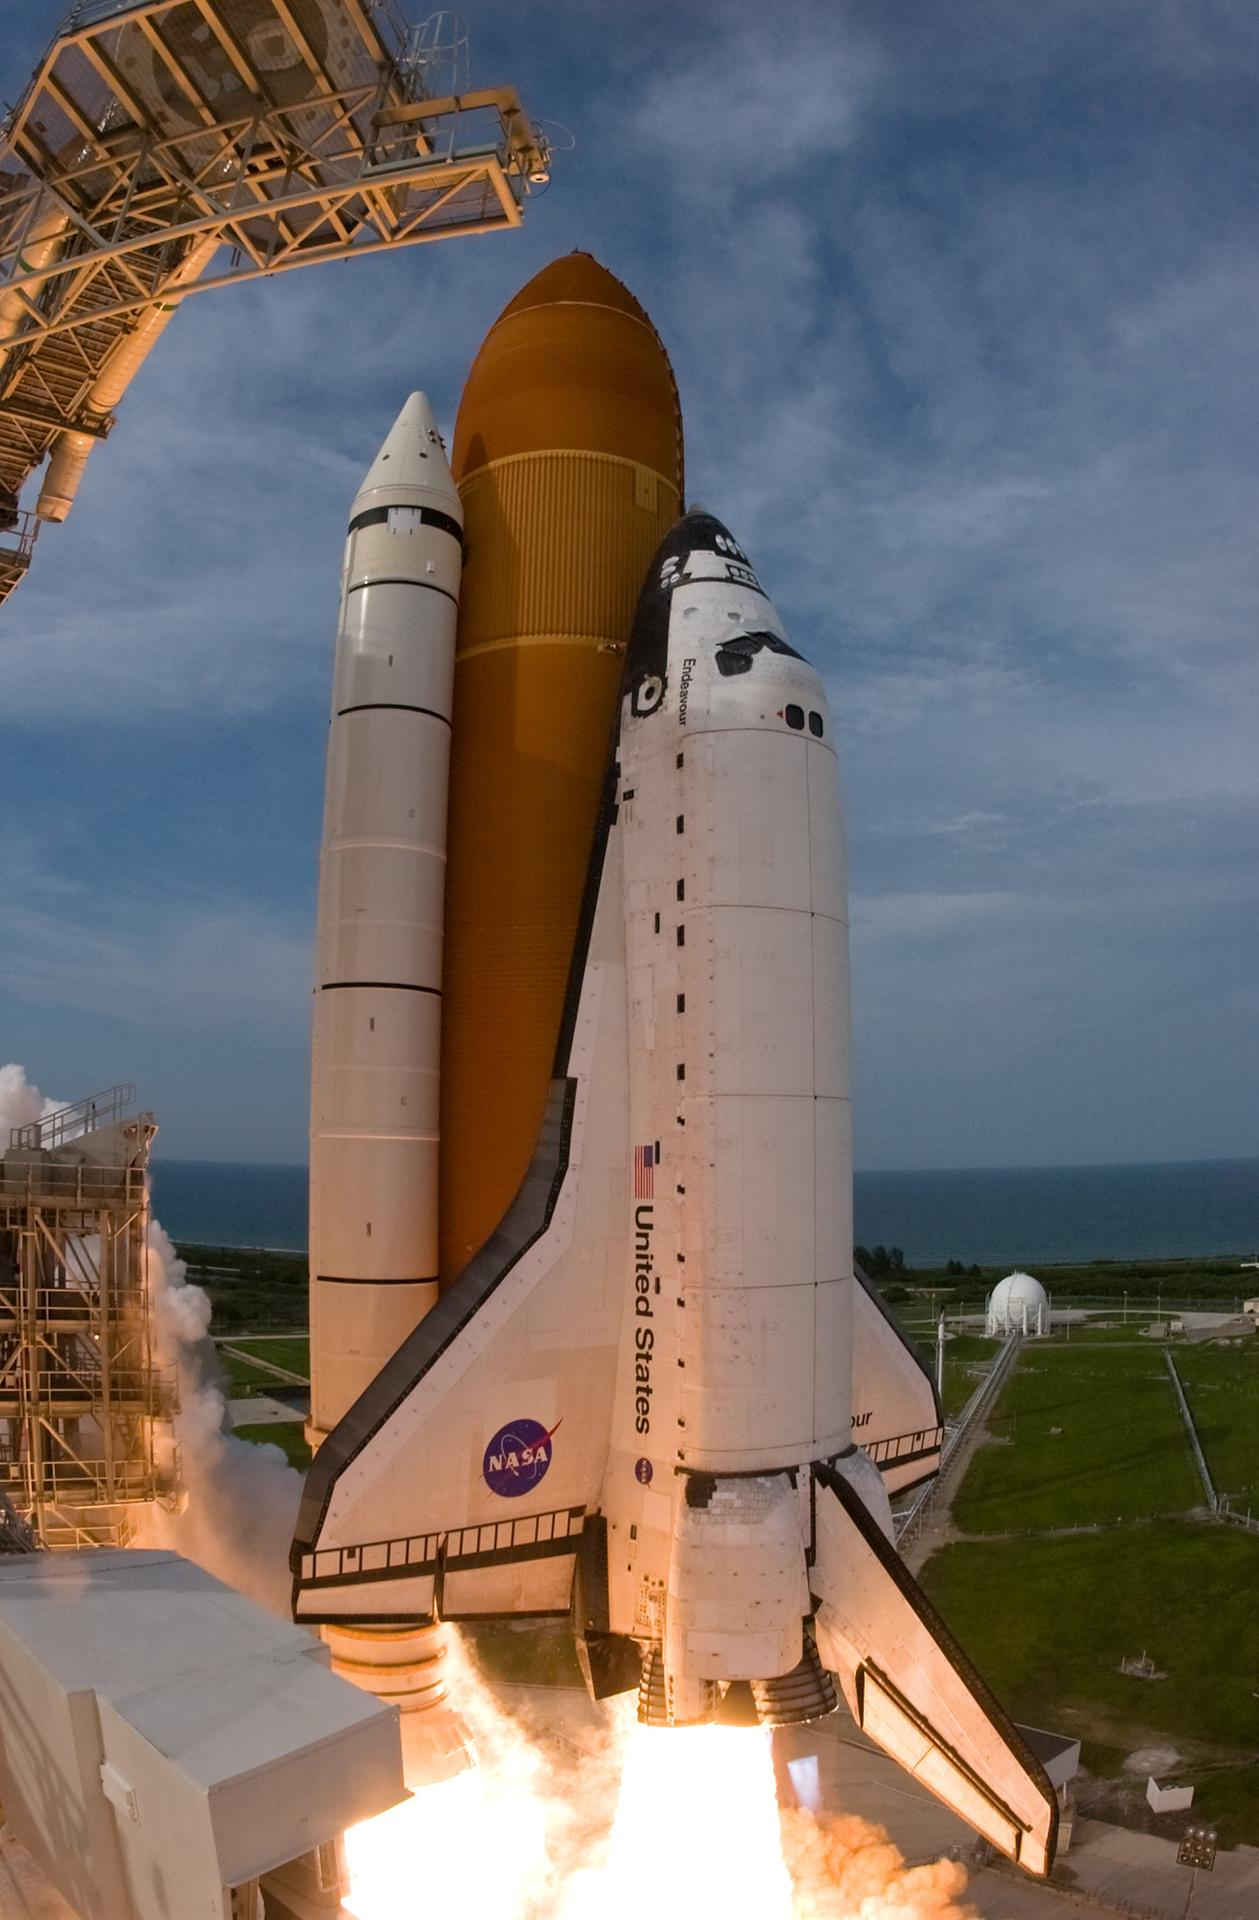
\includegraphics[width=.33\textwidth]{sts_foto.jpg}
   % \caption{Discovery taking off for its 35th time to assemble parts of the \acrshort{iss}}
   % \label{fig:discovery_photo}
\end{wrapfigure}

	Operated by \acrshort{nasa} from 1981 to 2011, the Space Shuttle was the first reusable space transportation system, an innovative orbital vehicle that combined the characteristics of a rocket and an airplane.
 
The Space Shuttle program enabled numerous scientific and technical missions, including the launch of satellites, the construction, maintenance of the \acrfull{iss} and a variety of scientific experiments in orbit.
This vehicle allowed astronauts and payloads to be transported into space and returned to Earth, marking a turning point in the history of astronautics.

The launch system consists of three RS-25 (\acrshort{ssme}) and two additional \acrfull{srb}. The \acrfull{ssme} was one of the most advanced and crucial technological elements of the \acrshort{sts}. The \acrshort{ssme}s were the primary rocket engines, propelled by \acrfull{lh2} and \acrfull{lox}, providing the necessary thrust for the Shuttle's liftoff and initial ascent to low Earth orbit. These engines were known for their efficiency and reliability, being able to operate under extreme conditions and be reused for multiple launches.

    %The Space shuttle propulsion system consists of three space shuttle main engines (SSME) which draw liquid oxigen ($ LO_2 $) and \acrlong{lh2} ($ LH_2 $) from the external tank (ET).On the sides of the ET two solid rocket boosters are attached.To control the attitude of the orbiter, once it has reached space, two orbital manouvering system (OMS) engines and 44 reaction control systems (RCS) thrusters are used.The following is an analysis of the SSME's thermodynamic cycle and how the propulsive properties change when another fuel is used instead of $ LH_2 $. 

The purpose of this report is to initially size the real \acrfull{ssme} and then, based on the total impulse and burning time of this engine, to resize the engine while changing the fuel from \acrlong{lh2} to \acrfull{lch4}. 
This analysis anticipates a simplification of the system components and a reduction in the mass of the \acrfull{et} given that methane has a much higher density than hydrogen. 
%Additionally, the storage temperature of methane is very similar to that of oxygen, which could help avoid issues related to thermal exchange between the fuel and oxidizer tanks.
%\begin{wrapfigure}{l}{.35\textwidth}
 %   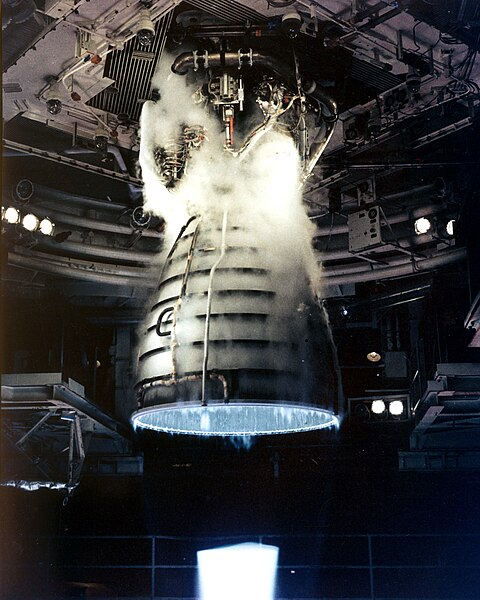
\includegraphics[width=0.33\textwidth]{ssmeTestFiring.jpg}
 %   \caption{a close-up view of a Space Shuttle Main Engine during a test firing}
  %  \label{fig:ssmetestfiring}
%\end{wrapfigure}
The path followed in this report involved taking upstream and downstream pressures of each component, the inlet temperatures to the various components, and the mass flow rates of the fuel and oxidizer.
Using these parameters, the turbopumps, injectors, combustion chamber, nozzle, and \acrlong{et} were appropriately sized through MATLAB. For the engine's performance analysis, NASA's \acrfull{cea} software was utilized.
\newacronym{of}{O/F}{Oxydizer to Fuel ratio}
Subsequently, by observing these performances and using the burning time, \acrfull{of}, total engine impulse, and combustion chamber pressure as starting points, the engine was resized for the new fuel (\acrshort{lch4}) by working backward from these parameters.


% TODO: (immagine del motore e del sistema di lancio dello shuttle) immagini da mettere una a destra e una a sinistra con il testo intorno

%\begin{figure}
%	\centering
 %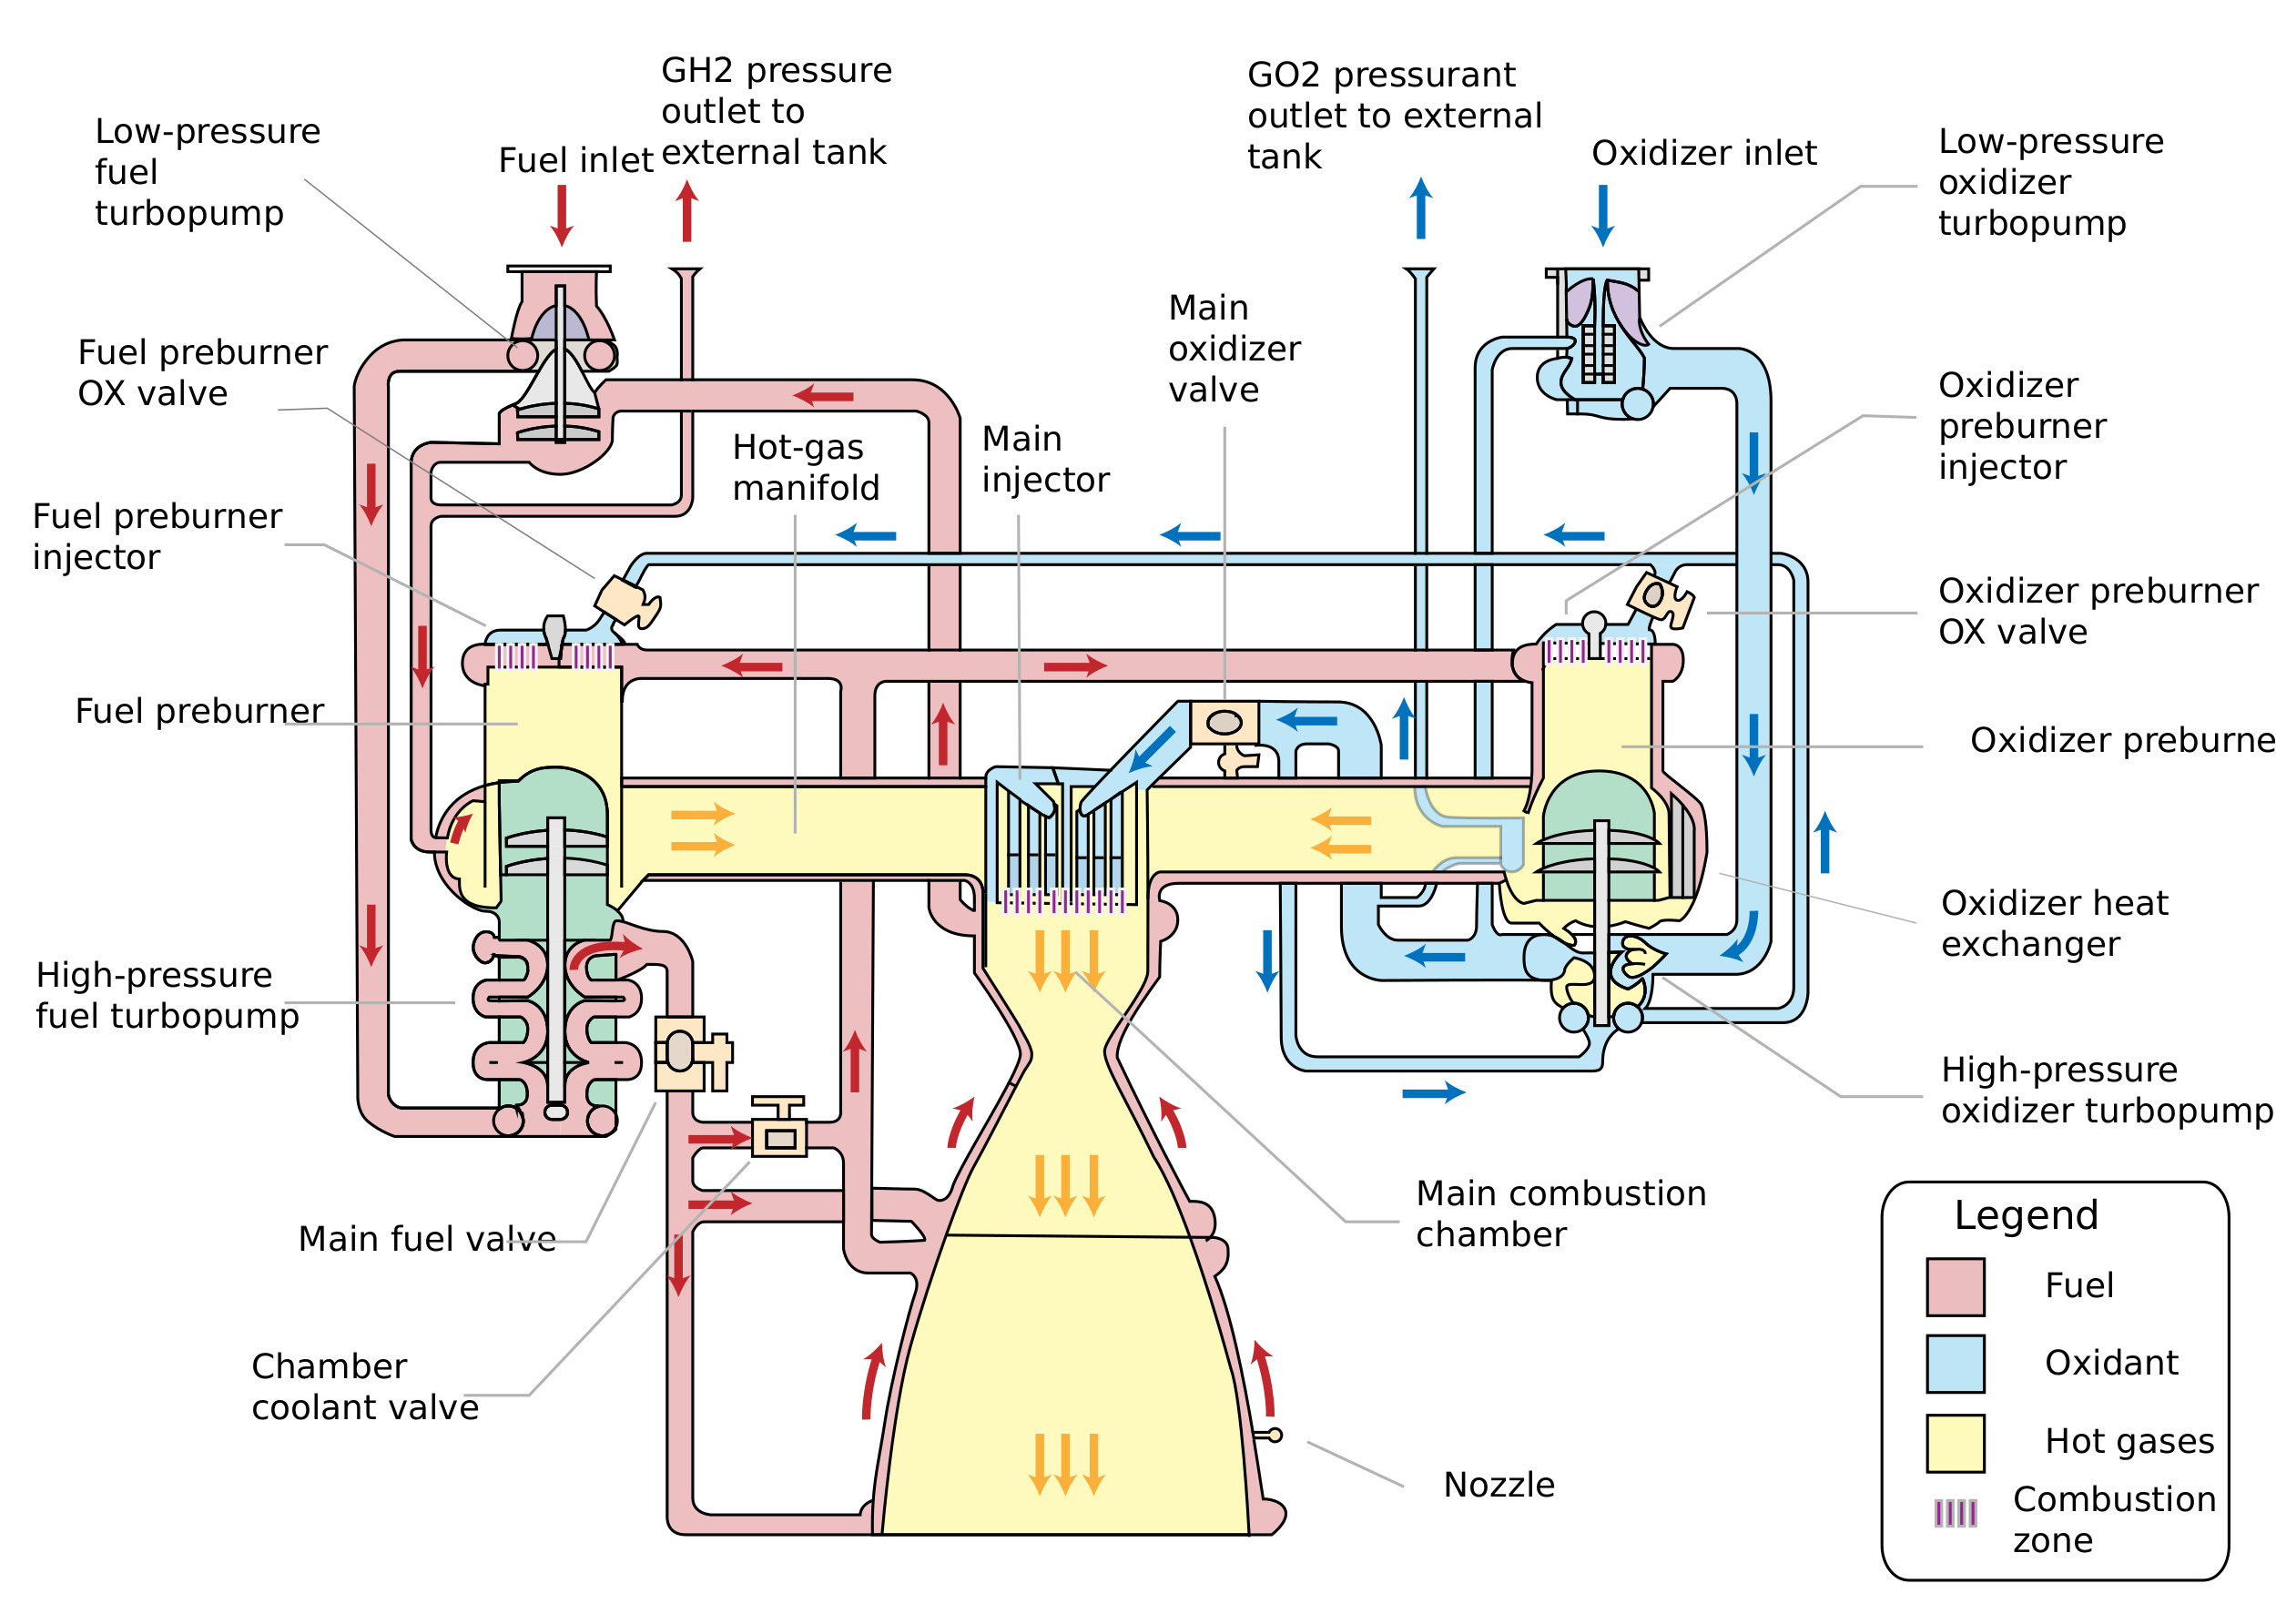
\includegraphics[width=.50\textwidth]{ssme_ciclo}
%	\caption{A functional diagram showing the flow of propellant through an RS-25 engine.}
%	\label{fig:ssme_cycle}
%\end{figure}
\subsection{Introduction to the staged combustion cycle}
The Stage Combustion Cycle used in the \acrfull{ssme} is a highly efficient system specifically designed for maximum performance.
In the \acrshort{ssme}, this cycle involves the partial combustion of both \acrlong{lh2} (fuel) and \acrlong{lox} (oxidizer) in separate preburners. 
The preburners produce hot, high-pressure, fuel-rich gases that drive the engine's turbopumps, which in turn feed the remaining propellants into the main combustion chamber at extremely high pressures.
What sets the \acrshort{ssme} apart is its use of a closed-cycle stage combustion process, where all the exhaust gases from the preburners are directed into the main combustion chamber, ensuring that no energy is wasted.
This results in very high efficiency, with the \acrshort{ssme} achieving one of the highest specific impulses of any rocket engine.
The high pressures and temperatures involved in this cycle make it extremely complex, but they also enable the \acrshort{ssme} to deliver the power needed for the Space Shuttle's demanding missions.
\begin{figure}[H]
	\centering
 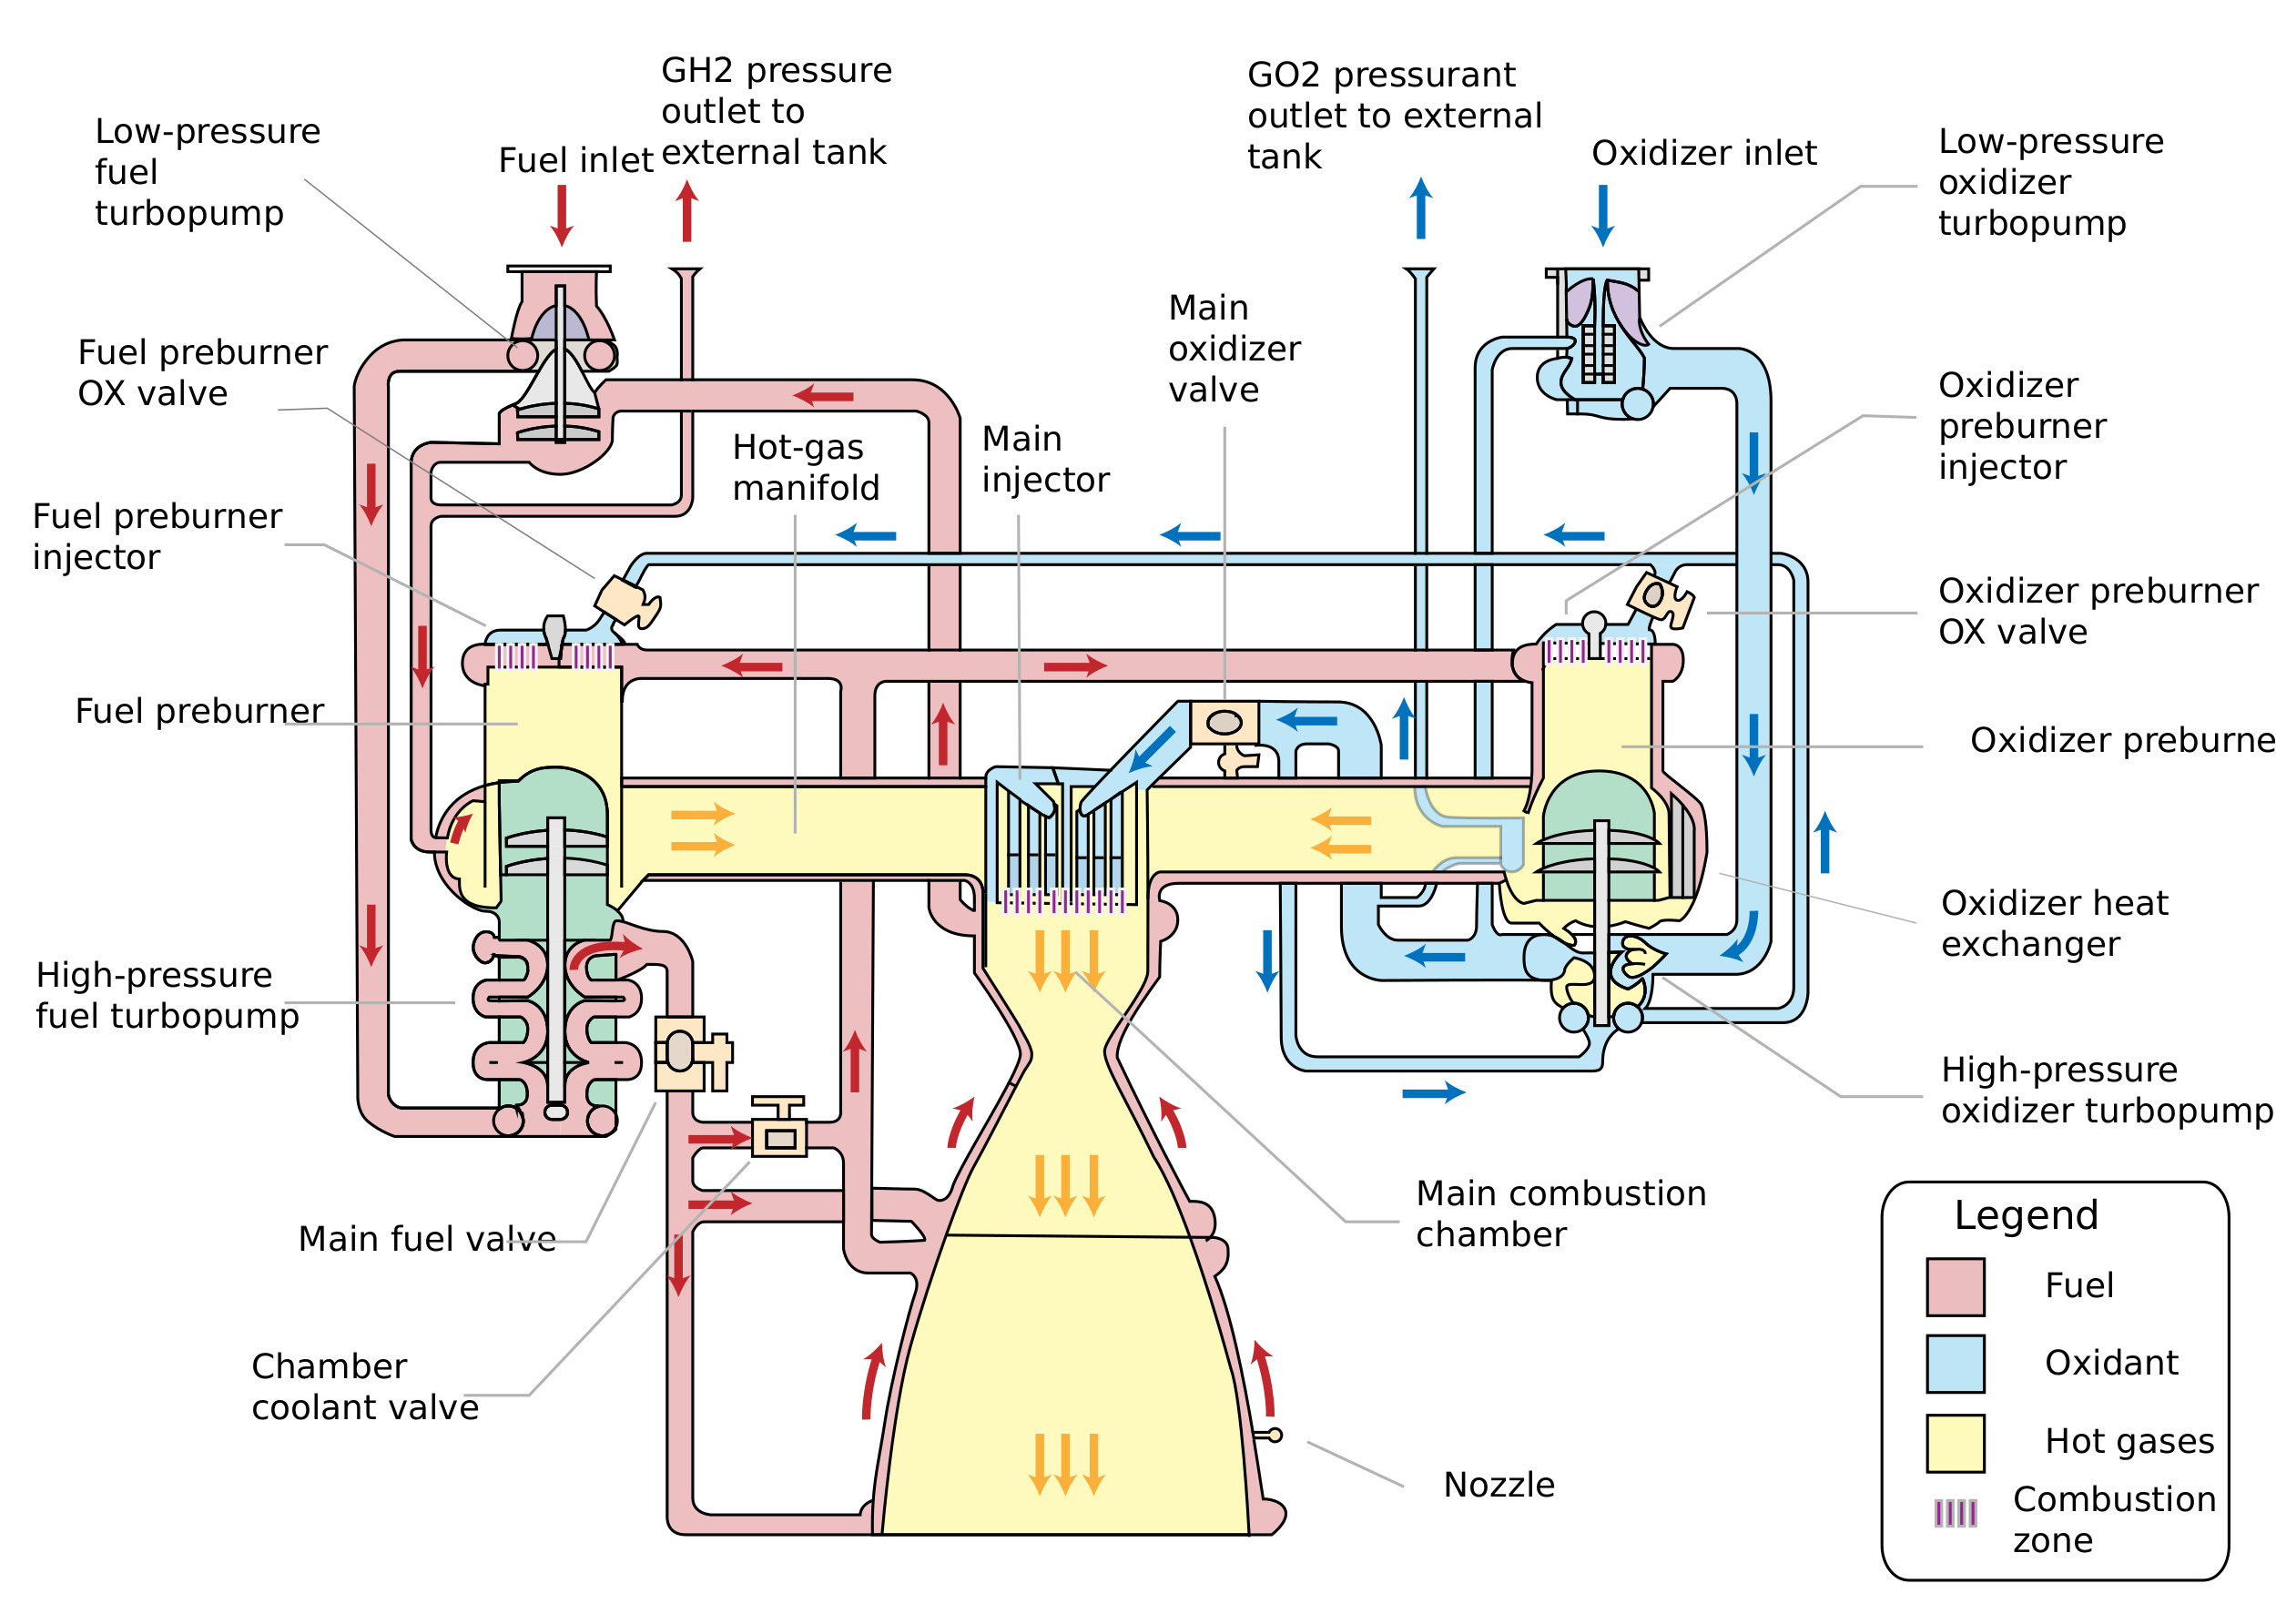
\includegraphics[width=.550\textwidth]{ssme_ciclo}
	\caption{A functional diagram showing the flow of propellant through an RS-25 engine.}
	\label{fig:ssme_cycle}
\end{figure}



\subsubsection{Brief description of liquid Oxygen Flow}

\acrlong{lox} enters the \acrfull{lpotp} at a pressure of approximately 0.2 MPa. It then flows through the low-pressure oxidizer duct and the \acrfull{hpotp}, where it is divided into a main flow and several branch flows. 
\newacronym{mov}{MOV}{Main oxidizer valve}
\begin{itemize}
    \item The main flow, comprising about 89\% of the total LOX, continues through the \acrfull{mov} and the main injector into the \acrfull{mcc}.
    \item A branch flow is directed to drive the \acrshort{lpotp} turbine. The discharge flow from this turbine is merged with the pump output flow, which is then routed to the \acrshort{hpotp}.
    \item Another branch supplies \acrshort{lox} to the heat exchanger coil, where it is gasified to pressurize the oxidizer tank in the \acrlong{et} and the pogo accumulator.
    \item A third branch, accounting for 11\% of the total \acrshort{lox}, supplies the preburner oxidizer boost pump located at the bottom of the \acrshort{hpotp}. This small pump increases the oxidizer pressure to approximately 48 MPa for injection into the preburners.
    \newacronym{opov}{OPOV}{Oxidizer Preburner Oxidizer Valve}    \newacronym{fpov}{FPOV}{Fuel Preburner Oxidizer Valve}
    \item The oxidizer flow is controlled by the \acrfull{opov} and the \acrfull{{fpov}}, which together determine the thrust level. The \acrshort{fpov} alone maintains a mixture ratio of 6.032 in the \acrshort{mcc}.
    \item Additional branches supply LOX to the three augmented spark ignition systems.
\end{itemize}

\subsubsection{Brief description of fuel Flow}
\newacronym{mfv}{MFV}{Main Fuel Valve}
The \acrfull{lh2} enters the \acrfull{lpftp} at a pressure of approximately 0.2 MPa. It flows through the low-pressure fuel duct, the \acrfull{hpftp}, and the high-pressure fuel duct, before passing through the \acrfull{mfv}. 

\begin{itemize}
    \item Up to this point, the fuel system is insulated. Beyond this point, the hydrogen is allowed to warm and gasify. The hydrogen then enters the diffuser, where the flow splits into three paths:
    \newacronym{hgm}{HGM}{Hot gas manifold}
        \begin{itemize}
            \item The first path (19\%) flows upward through 430 coolant channels in the \acrshort{mcc} and then drives the \acrshort{lpftp}. After exiting the \acrshort{lpftp} turbine, this branch supplies warm hydrogen gas to pressurize the fuel tank in the ET, with the remainder directed to both ends of the \acrfull{hgm}. The hydrogen then flows through the \acrshort{hgm} coolant spaces to enter a dedicated cavity in the main injector, from where it is injected into the \acrshort{mcc}.
            \newacronym{ccv}{CCV}{Chamber Coolant Valve}
            \item The second path (27.5\%) passes through 1,080 nozzle tubes, joining the third path (48.5\%) which bypasses the nozzle through the \acrfull{ccv}. The combined flow then splits to feed the preburners, with the fuel preburner receiving the majority (50\% vs. 26\%).
        \end{itemize}
\end{itemize}
The \acrlong{lch4} flow is maintained the same as the \acrlong{lh2}.

\subsection{Introduction to Liquid Hydrogen and Liquid Methane}
Liquid hydrogen is renowned for its exceptionally high specific impulse, which means it can generate more thrust per unit mass compared to other propellants.
This makes it ideal for missions where maximizing fuel efficiency is crucial. 
Hydrogen is particularly well-suited for use in advanced propulsion cycles like the staged combustion cycle employed by the \acrshort{ssme}, where the goal is to extract the maximum amount of energy from the propellant.
However, \acrlong{lh2} has a very low density (about 70.85 kg/m³ at 20.27 K), necessitating larger and heavier tanks to store the same amount of energy as denser fuels.
Furthermore, hydrogen must be stored at extremely low temperatures (around 20.27 K), which is significantly lower than the boiling point of \acrlong{lox} (90 K).
This substantial temperature difference presents considerable challenges in tank design and thermal management, increasing the risk of unwanted heat transfer between the fuel and oxidizer tanks.
Additionally, because hydrogen molecules are very small, they can easily escape through micro-cracks or porous materials, increasing the likelihood of leaks.

Liquid methane, in contrast, has a much higher density (about 422.62 kg/m³ at 100 K), allowing for a reduction in the volume of the tanks required to store the fuel, which in turn reduces the overall mass and size of the tanks.
Methane can be stored at a temperature close to that of \acrlong{lox} (100 K), which minimizes the challenges related to thermal management and reduces the risk of heat exchange issues between the fuel and oxidizer tanks.
Moreover, methane is easier to handle than hydrogen, as it does not require storage at extremely low temperatures and does not pose the same level of risk for leaks due to its larger molecular size.
However, methane has a lower specific impulse compared to hydrogen, meaning it is less efficient at converting fuel mass into thrust.
 Additionally, the combustion of methane can lead to the production of soot, which can complicate residue management and engine maintenance.

\section{Problem analysis}
The starting point for the analysis involves collecting data on pressures and temperatures from official documents \cite{file01}\cite{presentation}\cite{doc_4} found on the web for the staged combustion cycle of the RS-25, both upstream and downstream of the original engine components. 
This data is then used to size these components and calculate the engine's performance. 
In the second part of the analysis, the process is reversed: starting from the desired performance, the engine is sized for the new fuel. 
The sizing focuses on the turbopumps, preburners (injectors), combustion chamber, nozzle, and external tank, while simplified assumptions are made for other parts of the engine, such as engine cooling, heat exchangers, and feed lines.
 \subsection{Hypotesis}
 In this section are explained the assumptions made to simplify the design of the egnine: 

\begin{itemize}
\item\textbf{Properties of fluid:}

the fluids properties are determined using data obtained from the NIST Chemistry WebBook \cite{nist}.
    \item\textbf{Components of the engine excluded from this analysis:}

    In order the simplify the design carried out in this report the flex joints, the bearings, the LOX heat exchanger and the ignition system are not included in the design;

    \item\textbf{Nozzle and combustion chamber cooling system:}

    the cooling system of the nozzle is not sized in this report, however a factor for both fuel temperature rise and pressure drop along this system is considered during the analysis ;
    \item\textbf{Radius of the E.T.:}

    the diameter of the tank is set at $8.4 m$ , the measure of the real radius of the original E.T. ;
    %%TODO: qui cosa bisogna mettere?
    
\item\textbf{Thrust profile}:

    a simplifying assumption is made by considering the thrust profile to be constant throughout the motor's operation.
    This assumption allows for a more straightforward calculation, as the total impulse can be expressed as the integral of the constant thrust value multiplied by the burn time of the motor.


\end{itemize}

\subsection{Turbopumps design}
The Space Shuttle Main Engine (SSME) turbopump system consists of four main turbopumps, each playing a critical role in the engine's operation. These include the \acrfull{HPOTP} and the \acrfull{LPOTP}, as well as the \acrfull{HPFTP} and the \acrfull{LPFTP}. Together, these turbopumps increase the propellant pressure to extremely high levels, necessary for injection into the combustion chamber

%When designing a turbopump for space propulsion, several key parameters need to be calculated to ensure the pump operates efficiently and meets the specified requirements.
Given the known fluid characteristics and operational demands, the following equations are used to determine the design elements of the pump \cite{humble95}.

\subsubsection{Pump key design parameters}
\begin{itemize}
    
 \item\textbf{Pressure Differential and Head of the pump}

The pressure differential (\(\Delta P\)) across the pump is given by:
\begin{equation}
\Delta P = P_{\text{out}} - P_{\text{in}}
\end{equation}

The head (\(H\)) of the pump, which represents refers to the height to which a pump can raise a fluid. It represents the energy per unit weight of fluid imparted by the pump. The "head" is a way to describe the pressure that the pump can generate and is a key parameter in pump performance. It is calculated as:
\begin{equation}
H = \frac{\Delta P}{g_0 \cdot \rho}
\end{equation}
\nomenclature{$H$}{Head of the pump   [m]}
\nomenclature{\rho}{Density [$\frac{kg}{m^3}$]}
\nomenclature{$g_0$}{Gravitational acceleration [$\frac{m}{s^2}$]}
\item\textbf{Number of Stages}

The number of stages (\(N_s\)) required for the pump is determined based on the maximum theoretical pressure differential per stage (\(\Delta P_{\text{ps}}\)) and the overall pressure differential.
\nomenclature{$N_s$}{Number of stages   [-] }
\nomenclature{$\Delta P_{\text{ps}}$}{Maximum theoretical pressure differential    [MPa]}
This theoretical pressure differential per stage is set to 16 Mpa for the liquid hydogen while 47 Mpa for other cryogenic fluids \cite{humble95}.
\begin{equation}
N_s = \left\lceil \frac{\Delta P}{\Delta P_{\text{ps}}} \right\rceil
\end{equation}
where \(\lceil \quad \rceil\) denotes the ceiling function.

\item\textbf{Rotational Speed of the shaft}

The rotational speed (\(V_r\)) of the pump and turbine shaft is calculated using the stage specific speed (\(V_s\)) and the pump head divided by the number of stages:
\begin{equation}
V_r = \frac{V_s \cdot \left(\frac{H}{N_s}\right)^{0.75}}{\sqrt{Q}}
\end{equation}
\nomenclature{$V_r$}{Rotational speed   [m/s]}
where \(Q\) is the volumetric flow rate:
\nomenclature{$Q$}{Volumetric flow rate   [$\frac{m^3}{s}$]}
\begin{equation}
Q = \frac{\dot{m}}{\rho}
\end{equation}
\nomenclature{$\dot{m}$}{Mass flow rate  [kg/s]}
The stage-specific speed setting is based on extensive testing to ensure that the results closely match the data of the actual turbopumps.
For the pumps the elaborate \acrlong{lh2} the values of \(V_s\) are in the range (3 - 5), whilst for the pumps that use other cryogenic fluid (LOX and LCH4) the range is (2 - 6).

The rotational speed in revolutions per minute (rpm) is:
\begin{equation}
V_{rpm} = \frac{30 \cdot V_r}{\pi}
\end{equation}
\nomenclature{$V_{rpm}$}{Rotational speed in revolutions per minute  [rpm]}

\item\textbf{Outlet Temperature}

The outlet temperature (\(T_{\text{out}}\)) of the fluid is determined by adding the temperature change to the inlet temperature (\(T_{\text{in}}\)). The temperature change (\(\Delta T\)) is calculated using the enthalpic change and specific heat capacity (\(c_p\)):
\nomenclature{$c_p$}{Specific heat  [245]}
\begin{equation}
\Delta T = \frac{\Delta H}{c_p}
\end{equation}
where the enthalpic change (\(\Delta H\)) is:
\begin{equation}
\Delta H = \frac{P_{\text{req}}}{\dot{m}}
\end{equation}
and \(P_{\text{req}}\) is the power required to drive the pump:
\nomenclature{$P_{\text{req}}$}{Power required to drive the pump  [MW]}
\begin{equation}
P_{\text{req}} = \frac{g \cdot \dot{m} \cdot H}{\eta_{\text{pump}}}
\end{equation}
with \(\eta_{\text{pump}}\) being the efficiency of the pump.

Thus:
\begin{equation}
T_{\text{out}} = T_{\text{in}} + \Delta T
\end{equation}

\item\textbf{Power Required}

The power required (\(P_{\text{req}}\)) to drive the pump is given by:
\begin{equation}
P_{\text{req}} = \frac{g \cdot \dot{m} \cdot H}{\eta_{\text{pump}}}
\end{equation}
\nomenclature{$\eta_{\text{pump}}$}{Efficiency of the pump   [-]}
\end{itemize}

During the compression process of the \acrshort{HPFTP} it was observed that the fluid reached supercritical conditions. This transition to supercritical conditions lead to significant discrepancies between the theoretical results and the actual data. Supercritical fluids exhibit altered physical properties, which complicates the accuracy of a comprehensive pump analysis.

To address this issue and improve the precision of the results, a different approach was adopted only for this pump. Instead of analyzing the pump as a single unit, it was divided into its three distinct stages \cite{presentation}. This subdivision allowed for a detailed analysis of each stage individually.

By examining each stage separately, it was possible to have better control over the physical characteristics of the fluid throughout the various phases of the compression process. This approach facilitated the adjustment of design conditions to reflect the specific operational realities of each stage of the pump. Consequently, the results obtained were much closer to the actual experimental data, enhancing the reliability and accuracy of the pump design.

\subsubsection{Turbines key design parameters}

\begin{itemize}
    \item \textbf{Pressure Ratio}
    
    The pressure ratio is given by:
    \begin{equation}
    \beta = \frac{p_{\text{in}}}{p_{\text{out}}}
    \end{equation}
    \nomenclature{$\beta$}{Pressure ratio   [-]}

    \item \textbf{Power Required}
    
    The power generated the turbine is set equal to that of the respective pump, then is divided by the mechanical efficiency of both pump and turbine:
    \begin{equation}
    P_{\text{generated}} = \frac{P_{\text{p}}}{\eta_{\text{mech}}}
    \end{equation}
    \nomenclature{$\eta_{\text{mech}}$}{Total mechanical efficiency   [-]}
    \nomenclature{$\eta_{\text{turbine}}$}{Turbine efficiency   [-]}
    where \( \eta_{\text{mech}} = 0.81 \) is the total mechanical efficiency, calculated as \( \eta_{\text{pump}} \times \eta_{\text{turbine}} \) with both efficiencies assumed to be \(0.9\).

    \item \textbf{Outlet Temperature} 
    
    The outlet temperature is calculated as:
    \begin{equation}
    T_{\text{out}} = T_{\text{in}} - \left(\eta_{\text{turb}} \times \left(T_{\text{in}} - T_{\text{out,id}}\right)\right)
    \end{equation}
    where \(T_{\text{out,id}}\) is the ideal outlet temperature determined by:
    \nomenclature{$T_{\text{out,id}}$}{Ideal outlet temperature   [K]}
    \begin{equation}
    T_{\text{out,id}} = T_{\text{in}} \left(\frac{1}{\beta}\right)^{\frac{\gamma - 1}{\gamma}}
    \end{equation}
    \nomenclature{$\gamma$}{Heat capacity ratio 
[-]}
    \item \textbf{Isoentropic Spouting Velocity} 
    
    The isoentropic spouting velocity, representing the velocity the turbine gas flow would have if expanded isoentropically from the turbine inlet to the outlet pressure, is calculated as:
    \begin{equation}
    C_0 = \sqrt{2 \cdot c_p \cdot T_{\text{in}} \left(1 - \left(\frac{1}{\beta}\right)^{\frac{\gamma - 1}{\gamma}}\right)}
    \end{equation}
    \nomenclature{$C_0$}{Isoentropic spouting velocity  [m/s]}

\item\textbf{Number of stages}

In this case the number of the turbines stages is extrapolated from references \cite{sutton01} \cite{presentation} that describes the turbines.
\end{itemize}
%da inserire tabella con i dati
\subsection{Preburners and injectors design}

The \acrfull{ssme} employs a sophisticated preburner system designed to efficiently initiate and sustain the combustion process in its main combustion chamber. The \acrshort{ssme} features two preburners: one for the \acrfull{lh2} and one for the \acrfull{lox}.

The preburners are essentially small combustion chambers where a portion of the propellant is burned to produce high-pressure, high-temperature gases. These gases are then used to drive the turbopumps that supply the main combustion chamber with propellants.
This staged combustion results in a highly efficient process where the majority of the propellant is burned in the main combustion chamber.

By utilizing this staged combustion technique, the \acrshort{ssme} achieves high performance and efficiency, which is critical for the demanding requirements of space shuttle launches.

\subsubsection{Preburners combustion: NASA CEA analysis}
For the combustion process within the preburners, the NASA's \acrshort{Cea} software was utilized to model and analyze the combustion characteristics under fixed enthalpy and pressure conditions. The software is configured to solve combustion problems by specifying the specific \acrfull{O/F}, which varied depending on whether \acrlong{LCH4} or \acrlong{LH2} is used as the fuel. The analysis incorporated the chemical species and their respective temperatures, which rae determined from previous pumps analyses.

 The software provides detailed information on the combustion products, their thermophysical properties and their mass fractions. 
 This analysis is crucial because the exhaust gases, after passing through the High-Pressure Turbopumps turbines (HPTP), enter the combustion chamber.
 Understanding the properties of these gases ensures that the combustion chamber operates efficiently and effectively under the conditions dictated by the preburner’s output.

\subsubsection{Injector design}
The selected injector type is a coaxial injector, where the oxidizer flows through a central core and the fuel flows in an annular ring surrounding the core. 
This design is considered highly efficient for cryogenic fluids \cite{sutton01}. 
The coaxial configuration ensures optimal mixing and combustion efficiency by leveraging the high efficiency of the coaxial injector design for cryogenic propellants.

Given the mass flow rates of \acrfull{lox} and fuel \cite{presentation}, their densities, and the pressure differentials across the injectors, this analysis aims to determine the number and size of injectors needed to achieve the desired mass flow rates for both propellants.

Initially, the areas for LOX and fuel injectors are set to \(5 \times 10^{-6}\) m² and \(1 \times 10^{-5}\) m², respectively. These values serve as starting points for the calculations. A convergence tolerance of \(1 \times 10^{-10}\) and a maximum of 1000 iterations are defined to ensure accurate results.

The process involves iteratively refining the injector areas until convergence to the required mass flow rates is achieved or the maximum number of iterations is reached.


In each iteration, the exit velocities of LOX and fuel are calculated using the pressure differential and densities. The velocity is determined by the formula:
\begin{equation}
V = \sqrt{\frac{2 \cdot \Delta P}{\rho}}
\end{equation}
The mass flow rate through each injector is then computed using these velocities and the current injector areas.

Based on the mass flow rates of LOX and fuel, the number of injectors required is calculated.
This is done by dividing the total mass flow rate by the mass flow rate of a single injector and then taking the ceiling of the maximum value to ensure an adequate number of injectors.

New injector areas are calculated based on the desired mass flow rates and the number of injectors.
The new area for each injector is given by:
\begin{equation}
\text{New injectors area} = \frac{\dot{m}}{(\text{Number of injectors} \times \rho \cdot V)}
\end{equation}

The loop terminates when an area is reached such that the mass flow rate passing through that injector area satisfies the imposed tolerance requirement.

Upon convergence, additional parameters are calculated:
\begin{itemize}
    \item \textbf{Diameter of LOX Injector}: 
    
    Determined using the formula for the area of a circle: \begin{equation}
D_{\text{LOX}} = \sqrt{\frac{4 \cdot A_{\text{LOX}}}{\pi}}
\end{equation}
    \item \textbf{Thickness of fuel injector ring}: 
    
    Calculated as: \begin{equation}
\text{Thickness}_{\text{fuel}} = \sqrt{\frac{A_f + A_{\text{LOX}}}{\pi}} - \frac{D_{\text{LOX}}}{2}
\end{equation}
\end{itemize}

\subsection{Combustion chamber and main injector design}
\newacronym{mcc}{MCC}{Main Combustion Chamber}
The \acrfull{mcc} plays a critical role in rocket propulsion systems by performing several essential functions:

The design of the main combustion chamber involves calculating key geometric parameters to ensure optimal performance. The chamber consists of a converging section that compresses the flow, a throat where the flow reaches sonic conditions, and a diverging section where the gas expands.
In this document, the equations used for determining the dimensions of these sections are outlined and a visual representation of the combustion chamber profile is provided.

\subsubsection{Geometric Parameters}

The following equations are used to determine the critical dimensions of the combustion chamber:

\begin{itemize}

\item\textbf{Cross-sectional area of the combustion chamber (\( A_c \)):}
\nomenclature{$A_c$}{Cross-sectional area of the combustion chamber   [m^2]}
is given by:
\begin{equation}
A_c = \frac{\pi D_c^2}{4}
\end{equation}
where \( D_c \) is the diameter of the combustion chamber.
\nomenclature{$D_c$}{Diameter of the combustion chamber  [m]}
     \item \textbf{Combustion Chamber Volume (\(V_c\)) and Length (\(L_c\)):}
     \nomenclature{$V_c$}{Combustion chamber volume   [m^3]}
     \nomenclature{$L_c$}{Combustion chamber length    [m]}
            \begin{equation}
            V_c = L^* \cdot A_t
            \end{equation}
            \begin{equation}
            L_c = \frac{V_c}{A_c}
            \end{equation}
            where \(L^*\) is the specific length and is set to be 1.14 m for both the classic RS-25 nozzle and the modified engine's one.
            The throat area is calculated in the nozzle section in \cref{eq:throat_area}.

\item\textbf{The exit area of the combustion chamber (\( A_{e_{cc}} \)):}
\nomenclature{$A_{e_{cc}}$}{Exit area of the combustion chamber    [m^2]}
is determined by the exit-to-throat area ratio (\( A_{e_{cc}}/A_t \)):
\nomenclature{$A_t$}{Nozzle throat area    [m^2]}
\begin{equation}
A_{e_{cc}} = A_t \times \frac{A_{e_{cc}}}{A_t}
\end{equation}
\end{itemize}

The corresponding diameters for the throat (\( D_t \)) and exit (\( D_{e_{cc}} \)) are calculated as:
\nomenclature{$D_t$}{Nozzle throat diameter   [m]}
\nomenclature{$D_{e_{cc}}$}{Nozzle exit diameter    [m]}

\begin{equation} V_c = L^* \cdot A_t
            \end{equation}
            \begin{equation}
            L_c = \frac{V_c}{A_c}\end{equation}
\begin{equation}
D_t = \sqrt{\frac{4 A_t}{\pi}}
\end{equation}
\begin{equation}
D_{e_{cc}} = \sqrt{\frac{4 A_{e_{cc}}}{\pi}}
\end{equation}

The length of the converging section (\( L_{\text{converging}} \)) is calculated as :
\nomenclature{$L_{\text{converging}}$}{Length of the converging section    [m]}
\begin{equation} V_c = L^* \cdot A_t
            \end{equation}
            \begin{equation}
 L_c = \frac{V_c}{A_c}\end{equation}

while the diverging section (\( L_{\text{diverging}} \)) is predefined based on design requirements:
\nomenclature{$L_{\text{diverging}}$}{Length of the diverging section    [m]}
\begin{align}
L_{\text{diverging}} &= 0.20 \, \text{m}
\end{align}

To visualize the profile, the converging section is modeled linearly, while the diverging section is shaped using a cosine function to ensure a smooth transition. The radius at any point in the diverging section is calculated using:
\begin{equation}
y_{\text{diverging}} = \frac{D_t}{2} + \left(\frac{D_{e_{cc}}}{2} - \frac{D_t}{2}\right) \times \frac{1 - \cos\left(\frac{\pi (x - L_{\text{converging}})}{L_{\text{diverging}}}\right)}{2}
\end{equation}




\subsubsection{Injector Design and Function}
\newacronym{hgm}{HGM}{Hot Gas Manifold}
The main injector is a crucial component that integrates several fluid streams to achieve optimal combustion within the \acrfull{mcc}. It combines hot, fuel-rich gas from the preburners, cold hydrogen gas from the cooling circuits, and cold \acrlong{lox} from the \acrfull{hpotp}. The injector is centrally welded into the \acrfull{HGM}, creating passageways that allow these fluids to enter the appropriate cavities within the injector.

The injector is equipped with coaxial elements, just as the preburners injectors, each designed to handle specific fluid streams:

\begin{itemize}
    \item \textbf{Liquid Oxygen Injection:} 
    
    Each coaxial element injects \acrlong{lox} from the oxidizer manifold through its central post.
    \item \textbf{Hot Fuel-Rich Gas Injection:}
    
    The same elements also inject hot, fuel-rich gas from the preburners through their annulus, which is the cavity between the heat shield and the secondary plate.
    \item \textbf{Cold Hydrogen Gas:}
    
    Cold hydrogen gas, which has previously circulated through the double walls of the \acrshort{HGM}, enters the slot between the secondary plate and the lip of the primary plate. Both plates are porous and transpiration-cooled by this cold hydrogen gas as it flows through them.
\end{itemize}

The sizing of the injectors is carried out with the same equations utilized for the preburners injectors.

Flow shields are bolted to the outer row of injector elements.
These shields are designed to protect the elements from damage and erosion caused by the high-velocity gas. 
They are beyond the purpose of this project so they are not designed in this report.


\subsection{Performances calculation} \label{sec:perf}
The performance analysis of the engine is conducted for both hydrogen and methane fuels using NASA's \acrfull{cea} software. 
The problem is set up as a "rocket" analysis, utilizing known parameters such as the combustion chamber pressures and the expansion ratio. 
Regarding the combustion chamber pressures, the values for hydrogen are taken from official documentation of classic engine (19.7 Mpa) \cite{presentation}, while for methane, estimates are derived based on observations from the RS-25 engine and the SpaceX Raptor engine (21.5 Mpa) , the latter being a methalox engine.

Considering the expansion ratio, it is set to the original value used for the RS-25 engine \cite{data_sheet}, which is \(\varepsilon = 69\), for both hydrogen and methane cases.
\nomenclature{$\varepsilon$}{Nozzle expansion ratio     [-]}
This consistent expansion ratio allows for a comparative analysis of engine performance under similar operational conditions. 
The \acrshort{cea} software provides insights into the thermodynamic properties and performance metrics, such as specific impulse and thrust, which are essential for evaluating the efficiency and effectiveness of the propulsion system.

In the combustion analysis performed using NASA's \acrshort{cea} software, the chemical species are selected to accurately represent the real combustion environment.
For the fuel component, the products of combustion from the preburners are used, reflecting the actual gases that participate in the main combustion process.
These preburners combustion products are specifically chosen to capture the true chemical composition and thermodynamic properties of the gases involved. 
As for the oxidizer, \acrlong{lox} is used, in almost the same amount (380 kg/s) both in the original RS-25 and the LOX/LCH4 one.


\begin{table}[H]
    \centering
    \begin{minipage}{0.45\textwidth}
        \centering
        \begin{tabular}{|c|c|c|}
            \hline
            \textbf{TYPE} & \textbf{SPECIES} & \textbf{MASS FRACTION} \\
            \hline
          FUEL & $H_2$ & 0.52 \\
            \hline
             FUEL & $H_2$O & 0.48 \\
            \hline
            OXIDIZER & $O_2$ & 1 \\
            \hline
        \end{tabular}
        \caption{chemical species entering the main injector, case LOX/LH2}
        \label{tab:tabella1}
    \end{minipage}\hfill
    \begin{minipage}{0.45\textwidth}
        \centering
        \begin{tabular}{|c|c|c|}
            \hline
            \textbf{TYPE} & \textbf{SPECIES} & \textbf{MASS FRACTION} \\
            \hline
             FUEL & $CH_4$ & 0.29172 \\
            \hline
            FUEL & CO & 0.43602 \\
            \hline
            FUEL & C(gr) & 0.0947 \\
            \hline
            FUEL & $H_2$ & 0.08907 \\
            \hline
           FUEL & $H_2$O & 0.06766 \\
            \hline
            FUEL & $CO_2$ & 0.02083 \\
            \hline
            OXIDIZER & $O_2$ & 1 \\
            \hline
        \end{tabular}
        \caption{Chemical species entering the main injector, case LOX/LCH4}
        \label{tab:tabella2}
    \end{minipage}
    
\end{table}

    

In the combustion analysis for both hydrogen and methane, the oxidizer-to-fuel (O/F) ratios are chosen based on specific references to ensure realistic and accurate performance evaluations.
For hydrogen, an O/F ratio of 6.032 \cite{data_sheet} is used, which corresponds to the value specified for the original engine design. 
This ratio reflects the optimal conditions for hydrogen combustion in the given engine configuration. 
In contrast, for the methane case, an O/F ratio of 3 is utilized, as documented in the literature \cite{sutton01}.
This ratio is representative of the typical conditions used in methane-based propulsion systems and provides a comparative basis for evaluating the performance of methane versus hydrogen as propellants.
These O/F ratios are crucial for determining the combustion efficiency and overall engine performance in the analysis.
This setup ensures that the analysis accurately represents the combustion conditions and provides relevant performance metrics for both hydrogen and methane fuels.
The outputs from the NASA \acrshort{Cea} software that are utilized in the analysis include several key parameters: specific impulse, characteristic velocity, speed of sound at the nozzle exit, and the pressures and temperatures at the combustion chamber, throat, and exit sections. 
From the exit pressure, it is possible to infer the altitude at which the engine operates at optimal expansion. Additionally, important data regarding the combustion products were obtained, such as their density, specific heat capacity (\(c_p\)), specific heat ratio (\(\gamma\)) and molecular mass of the exhaust gases (\(M_m\)).
These outputs provide crucial information for understanding the engine's performance and the behavior of the exhaust gases under various conditions.
\nomenclature{$M_m$}{Molecular mass   [$\frac{kg}{kmol}$]}

Using the data obtained from the NASA \acrshort{cea} software, it is possible to calculate key performance metrics for the engine.
The exhaust velocity (\(V_e\)) at the nozzle exit is calculated using the following equation:
\nomenclature{$V_e$}{Exhaust velocity at the nozzle exit    [m/s]}

\begin{equation}
V_{e} = \sqrt{\left(\frac{2 \gamma}{\gamma - 1}\right) R T_{c} \left(1 - \left(\frac{p_{e}}{p_{c}}\right)^{\frac{\gamma - 1}{\gamma}}\right)}
\end{equation}

where \( \gamma \) is the specific heat ratio of the exhaust gases, \( R\) is the specific gas constant, \( T_{c} \) is the combustion chamber temperature, \( p_{e} \) is the exit pressure, and \( p_{c} \) is the combustion chamber pressure.
\nomenclature{$R$}{Specific gas constant   $[\frac{J} {Kg K}]$}
\nomenclature{$T_c$}{Combustion chamber temperature    [K]}
\nomenclature{$p_e$}{Exit pressure    [MPa]}
\nomenclature{$p_c$}{Combustion chamber pressure   [MPa]}

The thrust (\( T \)) produced by the engine is given by:
\nomenclature{$T$}{Thrust   [N]}
\begin{equation*}
     T = \dot{m}_{p} \cdot V_{e}
\end{equation*}

where \( \dot{m}_{p} \) is the mass flow rate of the propellant.
\nomenclature{$\dot{m}_p$}{Mass flow rate of the propellant   [ \frac{kg}{s}] }
Finally, the total impulse (\( I_{\text{tot}} \)) of the engine over the entire burn duration is calculated as:
\nomenclature{$I_{\text{tot}}$}{Total impulse   [N\cdot s]}
\begin{equation}
I_{\text{tot}} = T \cdot t_b
\end{equation}

It's important to note that the burning time ($t_b$) used in this calculation is 480 seconds \cite{link3}, corresponding to the original engine's burn duration.

The total impulse and the burning time are the starting point for the design of the engine using the methane.

\subsection{External Tank design}
In this section it is explored one of the areas of the design for which the modification of the propellants makes the biggest mark, the \acrfull{et}.
With the goal of maintaining the same uses and type of mission profiles possible it has been decided to estimate the volumes of the propellant utilizing the relation between specific impulse ($I_{\text{sp}}$) and total impulse ($I_{\text{tot}}$):
\nomenclature{$I_{\text{sp}}$}{Specific Impulse at sea level  [s]}
\begin{equation}
I_{\text{tot}} = I_{\text{sp}} \cdot g_0 \cdot m_{\text{prop}} \cdot 3 
\end{equation}
\nomenclature{$m_{\text{prop}}$}{Propellant mass   [Kg]}

%where
%\begin{itemize}
    %\item $I_{sp}$: specific impulse (at sea level)
   % \item $g_0$: earth gravity constant
   % \item $m_{prop}$: the propellant mass 
%\end{itemize}
%Since three RS-25s are contributing to the thrust we need to multiply the right side of the equation by three.
%While the specific impulse for the RS-25 is obtained with the NASA's Cea software analysis, we must calculate the total impulse. We can do that by using the following equation:
%\begin{equation}

 %   I_{tot} = T \cdot burning_time

%\end{equation}
%where $T$ represents the thrust in Newtons and the burning time is the same as in \cref{sec:perf} (measured in seconds). 
After obtaining the propellant mass ($m_{\text{prop}}$):
\begin{equation} 
m_{\text{prop}} = 3 \cdot \frac{I_{\text{tot}}}{I_{\text{sp}} \cdot g_0}
\end{equation}
Then the oxidizer and fuel mass can be estimated using the optimal O/F ratio for that specific combination, finding the mass of the oxidizer and the fuel used for propulsion purposes.
Unfortunately the tank must hold more than solely the propellants masses used to generate thrust and the total volume of the tank is a sum of different volumes:
\begin{equation}
V_{\text{tank}} = V_{\text{pu}} + + V_{\text{press}} +V_{\text{ullage}} + V_{\text{bo}} + V_{\text{trap}} 
\end{equation}
\nomenclature{$V_{\text{tank}}$}{Total tank volume    [m^3]}
\nomenclature{$V_{\text{pu}}$}{Usable propellant volume    [m^3]}
\nomenclature{$V_{\text{ull}}$}{Ullage volume   [m^3]}
\nomenclature{$V_{\text{bo}}$}{Boil-off volume  
 [m^3]}
\nomenclature{$V_{\text{trap}}$}{Volume of unusable propellant trapped  [m^3]}

Since an in depth analysis of feed lines and of the behaviours of cryogenic liquids inside the tank go beyond of this report, it is assumed that an increase of $2\%$ of the propulsion volume to hold $V_{\text{ull}}$, $V_{\text{bo}}$ and $V_{\text{trap}}$ is a sufficiently acceptable hypotesis.

\subsubsection{Autogenous tank pressurization system}
Both the fuel and the oxidizer tank, are pressurized by a part of the flow that exits the \acrshort{lpftp} and the \acrshort{lpotp} respectively \cite{presentation}. 
Such a system, in contrast with one that utilizes an inert gas (such as Helium) stored in a different tank, introduces a complication when calculating the volume of the tank, since it has to hold the pressurizer itself and the increased volume of the pressurizer must be considered when trying to find the volume of pressurizer necessary to pressurize the tank. 
The computation necessary is only possible with an iterative method. 
If the expansion process of the pressurizer gas is considered as an adiabatic process, since the burn duration is long (especially if compared to an attitude control, mono-propellant engine, where short bursts are necessary \cite{humble95}), it is possible to compute the final temperature of the tank when the pressurizer gas has fully expanded:
\begin{equation}
    T_f = T_{press} (\frac{P_{tank}}{P_{press}}) ^{\frac{\gamma_{press}-1}{\gamma_{press}}}
\end{equation}
\nomenclature{$T_f$}{Final pressure after pressurizer expansion in tank   [MPa]}

Subsequently it is imperative to proceed with the iterative method, after initializing the pressurizer volume to zero:
\begin{enumerate}
    \item Set $V_{\text{press}}$ as sum of $V_{\text{tank}}$ and $V_{\text{press}}$.
    \item Using the perfect gas law find the mass of the pressurizer from the volume stored in pressurized tank:
    \begin{equation}
        M_{\text{press}} = \frac{V_{\text{press}} \cdot P_{\text{tank}}}{R \cdot T_f }
    \end{equation}
    \nomenclature{$P_{\text{tank}}$}{Tank pressure   [MPa]}
    \nomenclature{$P_{\text{press}}$}{Pressure of the pressurizer gasses after heating    [MPa]}
    \nomenclature{$M_{\text{press}}$}{Mass of the pressurizer gasses    [kg]}
    \item Calculate the new value of $V_{press}$ occupied by the mass of the propellant in the tank:
    \begin{equation}
        V_{\text{press}} = \frac{M_{\text{press}} R T_{\text{tank}}}{P_{\text{tank}}} 
    \end{equation}
    \nomenclature{$T_{\text{tank}}$}{Temperature inside the tank  [K]}
    \item Repeat from step 1 until $V_{\text{press}}$ converges.
\end{enumerate}
Then add the resulting $V_{\text{press}}$ can be added to the $V_{\text{tank}}$, which represents the estimate for the volume of the needed propellants. 

\subsubsection{Tank shape and material}
The \acrlong{et} is composed of three components: oxidizer and fuel tanks and an intertank \cite{E_t}.
During the active life of the \acrshort{sts}, the materials used for the \acrlong{et} varied over time with the aim of reducing the dead weight of the tanks.
Since the aim of this report is to analyze the difference if methane is substituted to hydrogen, the intertank mass was disregarded and assumed to be the same mass, regardless the propellants utilized.
The whole structure was considered to be made of Al 2219-T8, the material used in the first iteration of the \acrlong{et}. Subsequent version, such as the \acrfull{lwt} and \acrfull{slwt} used better materials, managing to shave off $5000$ $kg$ of weight. 

Regarding the shape of the two tanks there are aerodynamic consideration to take in to account, especially for the oxidizer tank which has a ogive shape to reduce aerodynamic drag since it is situated at the top.
A simplified shape composed of a cylinder with two semi-spheres to its ends was analyzed in this report, which is also the shape that is considered to be lighter than a cylinder with an elliptical end \cite{humble95}.

This analysis begin with defining the tank burst pressure and a safety factor ($f_s$) of $2$ as suggested for pressurized tanks that hold a cryogenic fluid by R. Humble \cite{humble95}
\nomenclature{$f_s$}{Tank safety factor   [-]}
\begin{equation}
    p_b = P_{\text{tank}} \cdot f_s
\end{equation}
\nomenclature{$p_b$}{Tank burst pressure   [MPa]}
To better see the change in dimensions of the tank, the radius of the tank was kept the same and the height was taken as a free coordinate. 
The first step consisted of calculating the volume of the semi-spheres, although,  since two are present in each tank, one for each end of the cylinder, it possible to actually calculate for a sphere.
\begin{equation}
    V_{\text{sphere}} = \frac{4}{3} \pi r^3
\end{equation}
The thickness necessary to withstand the pressures of the tank was calculated in this manner:
\begin{equation}
    t_{\text{sphere}} = \frac{p_b \cdot r}{2F_{\text{allowed}}}
\end{equation}
\nomenclature{$F_{\text{allowed}}$}{Elastic Stress Permitted}
\nomenclature{$t_{\text{sphere}}$}{Thickness of the sphere   [m]}
and therefore the mass 
\begin{equation}
    m_{\text{sphere}} = A_{\text{sphere}} \cdot t_{\text{sphere}} \cdot \rho
\end{equation}
After finding the volume and mass of the sphere it is possible to  calculate the volume of the cylinder necessary to hold the propellant volume by a simple subtraction. The height of the tank was calculated:
\begin{equation}
    h_{\text{tank}} = \frac{V_{\text{cylinder}}}{\pi r^2} + 2r
\end{equation}
\nomenclature{$r$}{Radius of the External Tank  
 [m]}
\nomenclature{$h_{\text{tank}}$}{Height of the tank    [m]}
Then the necessary thickness of the cylinder was calculated:
\begin{equation}
    t_{cylinder} = \frac{p_b \cdot r }{F_{allowed}} 
\end{equation}
\nomenclature{$t_{\text{cylinder}}$}{Thickness of the cylinder    [m]}
and the mass was calculated in an analogous manner to that of the sphere.
Finally the masses, volumes and  height for the two propellants combinations were compared.
                             
\subsection{Nozzle Design and Profile Generation}
This section covers the design and dimensioning of the converging-diverging nozzle of the SSME, including a 2D and 3D profile generation
\subsubsection{Nozzle sizing}
The sizing process involves the use of the nozzle's performance parameters:

\begin{itemize}
    \item Specific impulse (\(I_{sp}\)) at sea level;
    \item Burn time: \(480 \, \text{s}\);
    \item Chamber pressure (\(p_c\));
    \item Exit pressure (\(p_e\));
    \item Chamber Temperature (\(T_c\)) ;
    \item Specific Velocity (\(c^*\)) ;

\end{itemize}
\nomenclature{$c^*$}{Specific velocity    [m/s]}
Given those data, the following calculations are performed to size the nozzle:
        \begin{itemize}
        \item\textbf {Throat area (\(A_t\)):}
        \begin{equation}
A_t = \frac{\dot{m}_p}{c^* \cdot p_c}
\label{eq:throat_area}
\end{equation}
            \item\textbf {Throat Diameter (\(D_t\)):} 
            
            is calculated from the throat area (\(A_t\)):
            \begin{equation}
            D_t = \sqrt{\frac{4 A_t}{\pi}}
            \end{equation}
            
            \item \textbf{Exit Diameter (\(D_e\)):}
            
            is obtained using the expansion ratio (\(\epsilon\)) and throat diameter:
            \begin{equation}
            A_e = \varepsilon \cdot A_t
            \end{equation}
            \begin{equation}
            D_e = \sqrt{\frac{4 A_e}{\pi}}
            \end{equation}
            
            \item \textbf{Combustion Chamber Volume (\(V_c\)) and Length (\(L_c\)):}
            \begin{equation}
            V_c = L^* \cdot A_t
            \end{equation}
            \begin{equation}
            L_c = \frac{V_c}{A_c}
            \end{equation}
            where \(L^*\) is the specific length and is set to be 1.14 m \cite{sutton01} for both the classic RS-25 nozzle and the modified engine's one.
            \nomenclature{$L^*$}{Specific lenght   [m]}
    \end{itemize}
              The length of the diverging and converging (combustion chamber) sections are scaled by a Bell factor \(K\). In this case, \(K = 0.75\). The adjusted lengths are:
              \nomenclature{$K$}{Bell factor   [-]}
    \begin{equation}
    L_c = L_c \times K
    \end{equation}
    \begin{equation}
    L_d = L_d \times K
    \end{equation}

\subsubsection{Nozzle Profile Generation}

The nozzle profile is generated using a MATLAB function that produces a converging-diverging nozzle shape.
The profile is divided into converging and diverging sections with the following characteristics:

\begin{itemize}
    \item \textbf{Converging Section:} The radius decreases linearly from the combustion chamber radius (\(R_c\)) to the throat radius (\(R_g\)). The radius as a function of the distance \(x\) along the converging section is given by:
    \nomenclature{$R_c$}{Combustion chamber radius   [m]}
    \nomenclature{$R_g$}{Throat radius   [m]}
    \begin{equation}
    y_{\text{conv}} = R_c - \left( R_c - R_g \right) \frac{x}{L_c}
    \end{equation}

    \item \textbf{Diverging Section:} The diverging section is modeled as a parabolic curve. The parabola's coefficients are calculated to ensure the profile transitions smoothly from the throat to the exit.
    The parabolic equation is:
    \begin{equation}
    y_{\text{div}} = a x^2 + b x + c
    \end{equation}
    where \(a\), \(b\), and \(c\) are determined by solving a system of equations that ensures the correct shape of the profile and the desired angle of divergence (\(\alpha_{\text{div}}\)).


To determine the convergent-divergent nozzle profile, the coefficients \(a\), \(b\), and \(c\) of the divergent parabola were calculated to satisfy the conditions at the throat and exit sections, including the slope at the throat determined by the divergence angle \(\alpha_{div}\). The system of equations is:

\begin{equation}
a R_g^2 + b R_g + c = 0
\end{equation}

\begin{equation}
a R_e^2 + b R_e + c = L_d
\end{equation}

\begin{equation}
2a R_g + b = \frac{1}{\tan(\alpha_{div})}
\end{equation}

Where:
\begin{itemize}
    \item $R_g$ is the radius at the throat section,
    \item \(R_e\) is the radius at the exit section,
    \item \(L_d\) is the length of the divergent section,
    \item \(\alpha_{div}\) is the divergence angle.
\end{itemize}
\nomenclature{$L_d$}{Length of the divergent section  [m]}
\nomenclature{$\alpha_{div}$}{Divergence angle  [deg]}

Once the 2D profile of the nozzle is determined, it is revolved around the central axis to create a 3D mesh. 
The points along the profile are rotated through 360 degrees to form the surface of the nozzle.

Finally, the generated 3D nozzle profile is visualized.
This provides an intuitive understanding of the nozzle's geometry and ensures that the design meets the required specifications.

\end{itemize}

\subsection{Modified RS-25 design}
The design of the modified RS-25 started with the idea of replying the total impulse of the original engine.
The other starting points are the burning time of the original engine, the O/F of 3 and the performances calculated with the analysis carried out with NASA Cea. Other hypotesis are made to complete the analysis:
\begin{itemize}
    \item\textbf{Temperature and pressure in the Tank:}

    those two data are taken looking up to the Raptor engine by SpaceX and were set to be 100 K and 0.2 Mpa ;

    \item\textbf{Pressures along the fuel line:} 
    
    the pressures along the tubes of the fuel line are estimated as almost equal to the case of LH2 engine so to simplify the analysis of the modified engine ;

    \item\textbf{Turbopumps characteristic:}
    
    the pressure rise and drop in the turbopumps are set to be similar to the LH2 turbopumps, same as the number of stages in the turbines. Also the type of pumps are not changed; 
    \item \textbf{Oxidizer line:}
    
    the oxidizer line is mantained the same as the one of the original RS-25, that because after the calculations of the masses flow nedeed to reach the required specific impulse it is noticed that it is almost equal to the mass flow in the line of the original engine;
    \item\textbf{Nozzle expansion ratio:}

    the nozzle expansion ratio is maintained equal to the one of the LH2 RS-25 nozzle to simplify the calculations;

    \item\textbf{Radius of the fuel tank:}

    the radius of the fuel tank is maintained equal to the LH2 tank. the dimension that is modified in the second analysis is the height of that tank;

    \item\textbf{Fluid properties: }

   The fluid properties are determined using data obtained from the NIST Chemistry WebBook \cite{nist}.
\end{itemize}

\section{Discussion of results}
\subsection{Classic RS-25}
\subsubsection{Turbopumps}
Comparing the performance data from the analysed engine with the real data for the actual RS-25  reveals notable differences, reflecting the impact of different design assumptions and operational conditions.


\begin{table}[H]
\centering
%\scriptsize
\begin{tabular}{|l|c|c|c|c|}
\hline
\textbf{Parameter} & \textbf{LPFTP} & \textbf{HPFTP} & \textbf{LPOTP} & \textbf{HPOTP} \\ \hline
\textbf{Pumps} & & & & \\ \hline
$N_{stages}$ [-] & 1 & 3 & 1 & 1 \\ \hline
$T_{out}$  [K] & 23.986 & 58.2935 & 92.0429 & 111.3328\\ \hline
$P_{req}$ [MW] & 2.4514 & 53.5435 & 1.199 & 15.7754 \\ \hline
$V_{rpm}$ [rpm] & 15319.8516 & 34360 & 3844.0483 & 22062.9075 \\ \hline
$H$ [m] & 2520.2092 & 58146.903 & 195.105 & 2272.8604 \\ \hline
\textbf{Turbines} & & & & \\ \hline
$N_{stages}$ [-] & 2 & 2 & 6 & 3 \\ \hline
$T_{out}$  [K] & 250.8699 & 807.6214 & - & 683.2951 \\ \hline
$P_{produced}$ [MW] & 2.7238 & 59.4928 & 1.3322 & 17.5282 \\ \hline
$V_{rpm}$ [rpm] & 15319.8516 & 34360 & 3844.0483 & 22062.9075 \\ \hline
$\beta$ [-]& 1.3424 & 1.5511 & 9.0797 & 1.5573 \\ \hline
$c_{0}$  [m/s] & 818.201 & 1275.5694 & 489.8449 & 1262.0115 \\ \hline
\end{tabular}
\caption{Turbopumps data, case LOX/LH2}
\label{tab:turbo_pump_ox_fuel}
\end{table}

\subsubsection{Preburners injectors design}

\begin{table}[H]
\centering
%\scriptsize
\begin{tabular}{|l|c|c|}
\hline
\textbf{Parametro} & \textbf{Fuel Preburner} & \textbf{Oxidizer Preburner} \\ \hline
Area Inj. LH2 [m²] & 9.9398 \times 10^{-6} & 9.7755 \times 10^{-6} \\ \hline
Area Inj. LOX [m²]& 1.3230 \times 10^{-6} & 8.3538 \times 10^{-6} \\ \hline
Thickness Fuel annulus [m] & 0.0012 & 0.0013 \\ \hline
Diameter LOX injector [m] & 0.0013 & 0.0010 \\ \hline
Number of elements  [-] & 202 & 114 \\ \hline
\end{tabular}
\caption{Preburners injectors data, case LOX/LH2}
\label{tab:preburner_data}
\end{table}

\subsubsection{Performances}

The Cea outputs considered are the ones under the hypotesis of "frozen composition".

The provided data details key performance parameters at the throat and exit 2 of the nozzle and compares them to the original Space Shuttle Main Engine (SSME).

The throat pressure is 19.753 MPa, slightly lower than the SSME's typical 20.7 MPa, showing a decrease of about 4.6\%. The exit pressure of 0.00017812 MPa reflects the expected significant drop in pressure.

The throat temperature of 3828.87 K is higher than the typical SSME value of 3500 K, with an increase of approximately 9.4\%. At the exit, the temperature drops to 1046.74 K, indicating a cooling of about 72.7\%.

The throat density of 11.590 kg/m³ is close to SSME values, with a variation of around 1\%. The exit density drops significantly to 0.038229 kg/m³, a decrease of about 99.7\%.

Specific heat capacity (Cp) and specific heat ratio (gamma) values are consistent with SSME's hydrogen-oxygen combustion products. Gamma increases from 1.1947 to 1.2808, showing a 7.2\% increase.

Sonic velocity at the throat is 1427.0 m/s, similar to SSME values. The Mach number at the exit is 4.354, indicating high supersonic flow.

Characteristic velocity is 2015.2 m/s, slightly lower than the SSME’s 2050 m/s, with a decrease of 1.7\%. The specific impulse at the exit is 379.20 seconds, about 3.4\% higher than the SSME's 366 seconds.

In summary, the data generally aligns with SSME performance, with minor variations likely due to specific design or operating conditions.

\twominisw{
\begin{table}[H]
\centering
%\scriptsize
\begin{tabular}{|l|c|c|c|}
\hline
\textbf{Parameter} & \textbf{Throat} & \textbf{Throat} & \textbf{Exit 2} \\ \hline
P [MPa] & 19.753 & 11.157 & 0.00017812 \\ \hline
T [K] & 3828.87 & 3486.35 & 1046.74 \\ \hline
$\rho$ [kg/m³] & 11.590 & 7.1896 & 0.038229 \\ \hline
Cp [kJ/(kg·K)] & 2.7308 & 2.6953 & 2.0304 \\ \hline
$\gamma$ & 1.1947 & 1.1978 & 1.2808 \\ \hline
Son. Vel [m/sec] & 1427.0 & 1363.4 & 772.5 \\ \hline
Mach Number & 0 & 1 & 4.354 \\ \hline
$\varepsilon$ & 0 & 1 & 69.000 \\ \hline
$C^*$ [m/sec] & 2015.2 & 2015.2 & 2015.2 \\ \hline
$C_T$ & - & 0.6766 & 1.8441 \\ \hline
$I_{sp}$ [s] & - & 139.122 & 379.20 \\ \hline
\end{tabular}
\caption{Performance Parameters and Thermodynamic Properties}
\label{tab:thermo_performance}
\end{table}
}{
\begin{table}[H]
\centering
%\scriptsize
\begin{tabular}{|l|c|}
\hline
Parameter & Mass Fraction \\ \hline
$H$ & 0.00099 \\ \hline
$HO_2$ & 0.00171 \\ \hline
$H2$ & 0.00520 \\ \hline
$H_2 O$ & 0.60696 \\ \hline
$H_2 O_2$ & 0.00028 \\ \hline
$O$ & 0.02379 \\ \hline
$OH$ & 0.12551 \\ \hline
$O_2$ & 0.23555 \\ \hline
$O_3$ & 0.00001 \\ \hline
\end{tabular}
\caption{Composition of exhaust gases, cas LOX/LH2}
\label{tab:mass_fractions}
\end{table}
}{.73}{.23}

\subsubsection{External Tank design}

Comparing the values obtained from the analysis to those of the actual Space Shuttle External Tank (ET) provides some insights into their relative performance. For LOX, the usable propellant volume is 560.0802 m³, which is comparable to the approximately 558 m³ of the real ET. The total volume excluding the pressurizer of 571.2818 m³ closely matches the real ET's 570 m³.
For hydrogen, the usable propellant volume is 1492.6473 m³, which is slightly larger than the real ET's 1450 m³, indicating a somewhat larger design in this model. The total volume excluding the pressurizer of 1522.5002 m³ is also larger compared to the real ET's 1500 m³.
The pressurizer volume in the model is 9.9759 m³ for LOX and 18.8586 m³ for hydrogen, which aligns well with real values, although specific values for the real ET may vary slightly.
The total tank height in this analysis does not consider the intertank height.

\begin{table}[h!]
\centering
%\scriptsize
\begin{tabular}{|l|c|c|}
\hline
\textbf{Parameter} & \textbf{Oxygen} & \textbf{Hydrogen} \\ \hline
Usable Propellant Volume [$m^3$]& 560.0802 & 1492.6473 \\ \hline
Total Volume Excluding Pressurizer [$m^3$] & 571.2818 & 1522.5002 \\ \hline
Pressurizer Volume [$m^3$] & 9.9759 & 18.8586 \\ \hline
Final Volume [$m^3$] & 581.2577 & 1541.3588 \\ \hline
Tank Mass [$Kg$] & 20952.795 & 20148.4189 \\ \hline
Tank Height [m] & 13.2887 & 30.6135 \\ \hline
\end{tabular}
\caption{External Tank data, case LOX/LH2}
\label{tab:propellant_data}
\end{table}

\subsubsection{Nozzle design and profile generation}
\twominisw{
\begin{table}[H]
\centering
%\scriptsize
\begin{tabular}{|l|c|}
\hline
\textbf{Parameter} & \textbf{Value} \\ \hline
$D_t$ [m] & 0.25 \\ \hline
$D_{e_{cc}}$ [m] & 2.10 \\ \hline
$V_c$ [$m^3$] & 0.06 \\ \hline
$L_c$ [m] & 0.36 \\ \hline
\end{tabular}
\caption{Nozzle Dimensions, case LOX/LH2}
\label{tab:nozzle_dimensions}
\end{table}
}{
\begin{figure}[H]
	\centering
 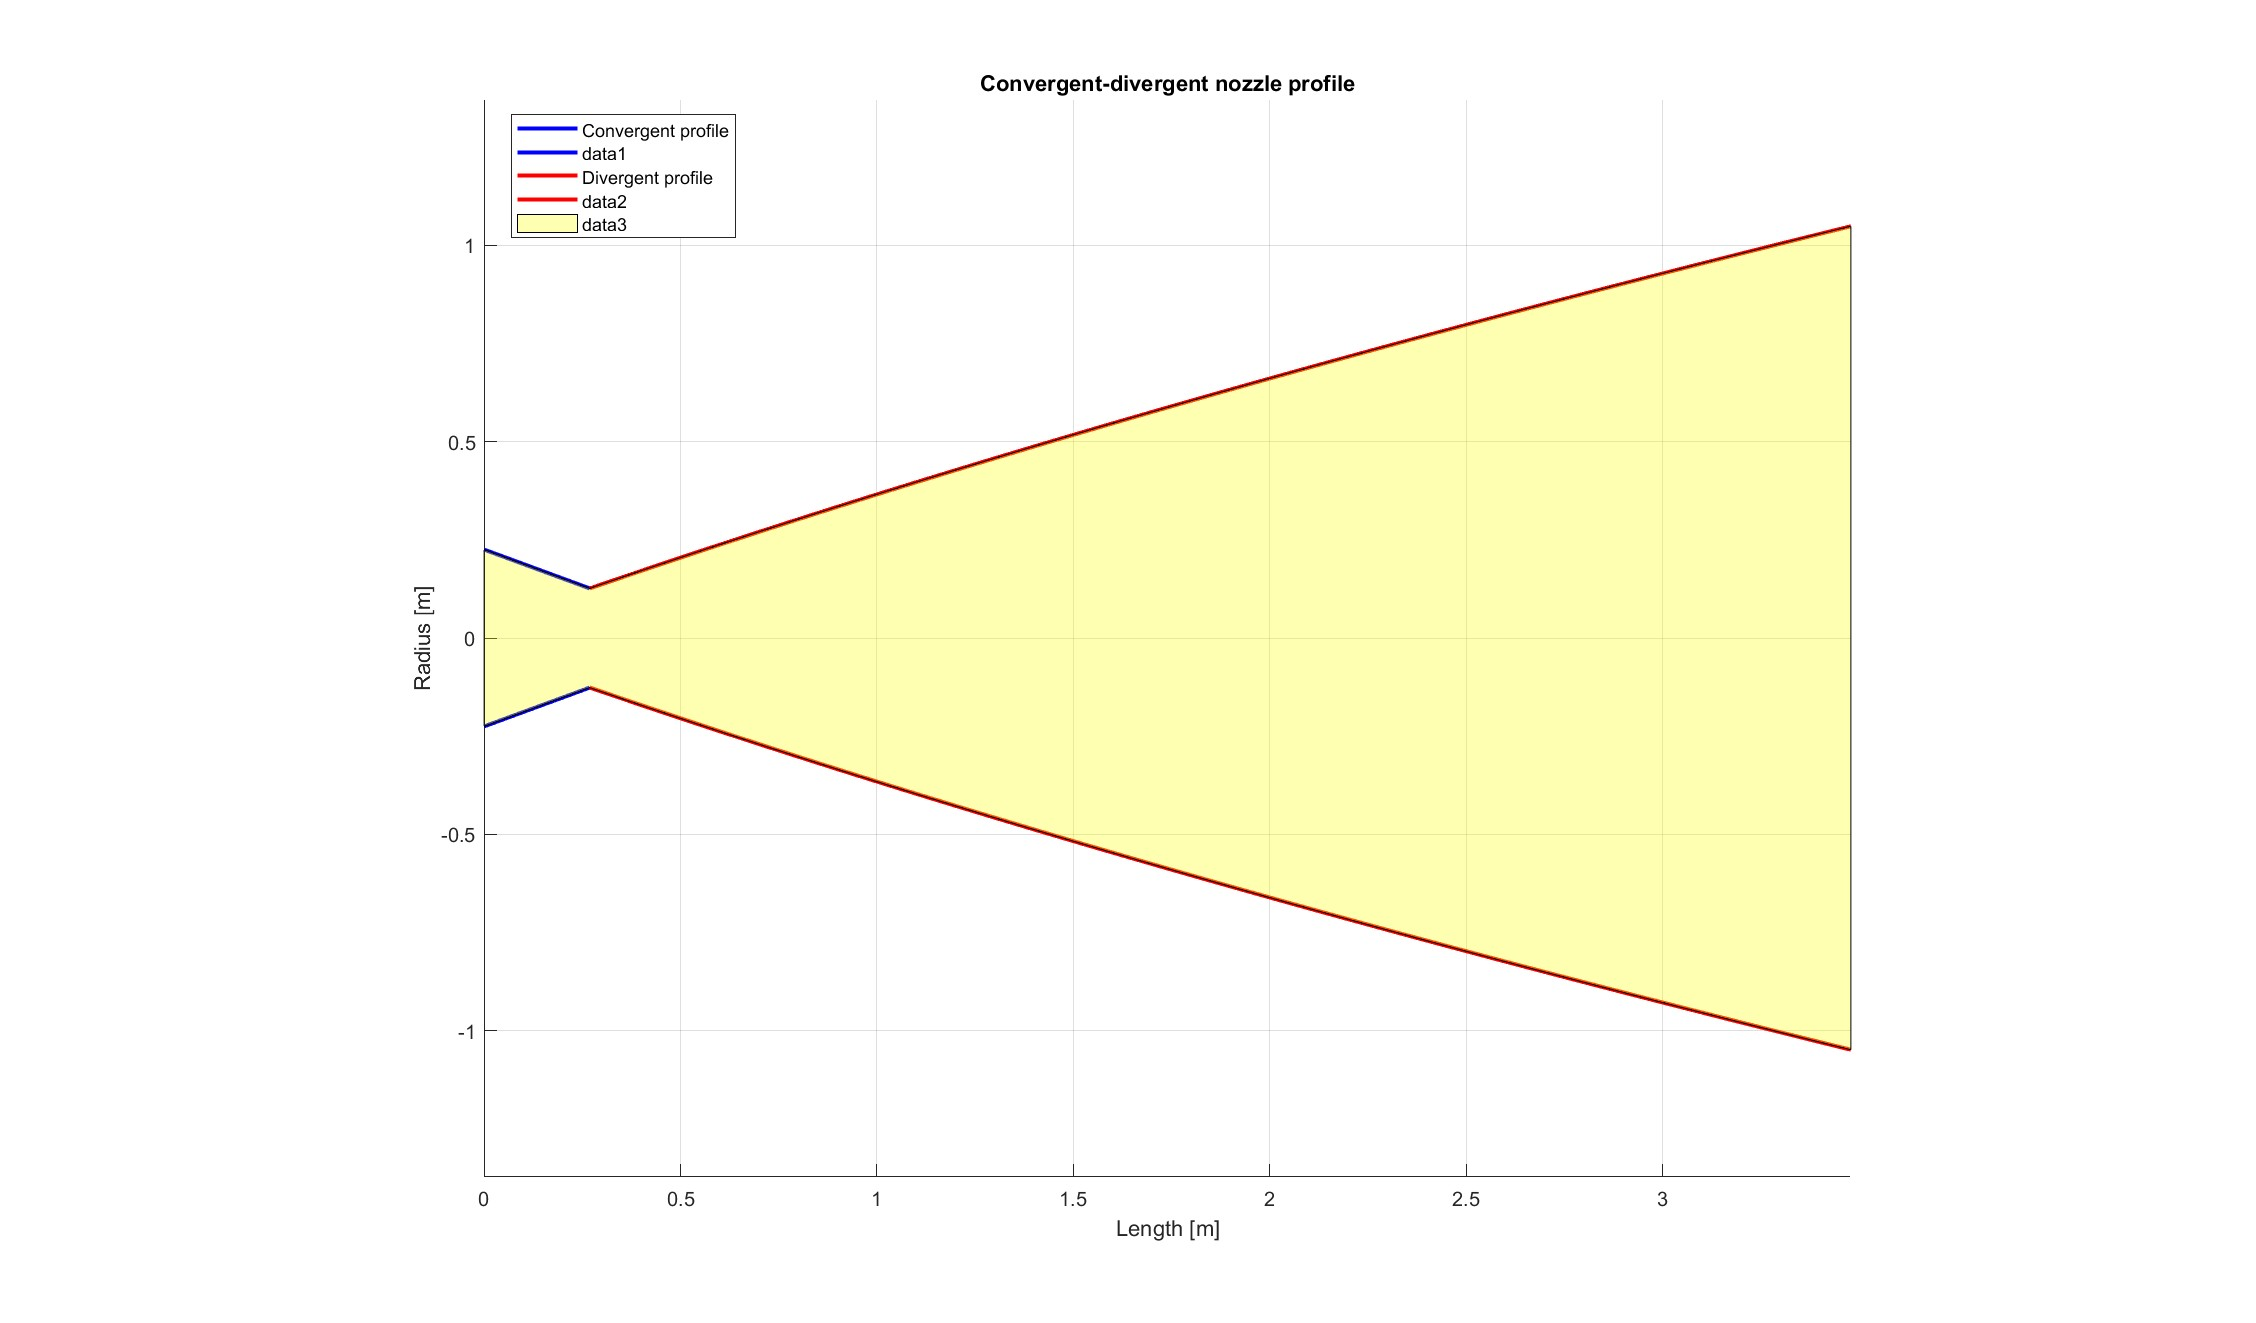
\includegraphics[width=.9\textwidth]{idrogeno_nozzle}
	\caption{Nozzle 2D profile, case LOX/LH2}
	\label{fig:idrogeno_nozzle}
\end{figure}
}{.18}{.80}
\subsection{Modified RS-25}
\subsubsection{Turbopumps design}
\subsubsection{Comparison with Methane Data}

Comparing the data for methane-based turbopumps and turbines with the previous hydrogen-based configuration reveals notable differences that simplify the design and operation of the system.

**Pumps**: The low-pressure fuel turbopump (LPFTP) for methane has a significantly lower power requirement of 0.55622 MW, compared to 2.4514 MW for hydrogen. This reduction of approximately 77\% suggests that methane's lower energy density allows for smaller and more efficient pumps. The output temperature for methane is 101.33 K, higher than the hydrogen temperature of 23.986 K, reflecting different thermal management needs. Additionally, the pump speed for methane is much lower at 2082.65 rpm compared to 15319.85 rpm for hydrogen, indicating a more stable and manageable operating condition.

Similarly, the high-pressure fuel turbopump (HPFTP) for methane operates at a reduced power of 14.5778 MW, about 73\% lower than the hydrogen configuration's 53.5435 MW. The output temperature is higher at 137.14 K compared to 58.2935 K, which simplifies the thermal design. The RPM values are more manageable for methane, suggesting less complex rotational dynamics.

**Turbines**: For methane, the low-pressure turbine has an output temperature of 277.83 K, higher than 250.87 K for hydrogen. This results in a slightly increased power production of 0.61802 MW compared to 2.7238 MW, reflecting different efficiency levels but a more controlled temperature range. The high-pressure turbine produces 18.2222 MW, a bit lower compared to the hydrogen engine’s 59.4928 MW, with a similar RPM, simplifying the design by reducing the power requirements and potentially lowering mechanical stresses.

Overall, using methane simplifies the design by reducing the power requirements and operational speeds of pumps and turbines, which results in a more compact and potentially more reliable system. The changes in temperature and power requirements indicate that methane-based systems could benefit from improved thermal management and more straightforward operational control compared to hydrogen-based systems.

\begin{table}[H]
\centering
%\scriptsize
\begin{tabular}{|l|c|c|c|c|}
\hline
\textbf{Parameter} & \textbf{LPFTP} & \textbf{HPFTP} & \textbf{LPOTP} & \textbf{HPOTP} \\ \hline
\textbf{Pumps} & & & & \\ \hline
$N_{stages}$ & 1 & 1 & 1 & 1 \\ \hline
$T_{out}$  [K] & 101.3278 & 137.1437 & 92.0429 & 111.3328 \\ \hline
$P_{req}$ [MW] & 0.55622 & 14.5778 & 1.199 & 15.7754 \\ \hline
$V_{rpm}$ [rpm] & 2082.6533 & 25419.41 & 3844.0483 & 22062.9075 \\ \hline
$H$ [m] & 327.2859 & 9061.0488 & 195.105 & 2272.8604 \\ \hline
\textbf{Turbines} & & & & \\ \hline
$N_{stages}$ & 2 & 2 & 6 & 3 \\ \hline
$T_{out}$  [K] & 277.8305 & 1475.0836 & - & 1476.7055 \\ \hline
$P_{produced}$ [MW] & 0.61802 & 18.2222 & 1.3322 & 17.5282 \\ \hline
$V_{rpm}$ [rpm] & 2082.6533 & 34360 & 3844.0483 & 22062.9075 \\ \hline
$\beta$ [-]& 1.3424 & 1.5504 & 9.0799 & 1.5504 \\ \hline
$c_{0}$  [m/s] & 516.5844 & 1389.0864 & 489.8449 & 1421.052 \\ \hline
\end{tabular}
\caption{Turbopumps data, case LOX/LCH4}
\label{tab:turbo_pump_ox_fuel}
\end{table}

\subsubsection{Preburners injectors design}

\begin{table}[H]
\centering
%\scriptsize
\begin{tabular}{|l|c|c|}
\hline
\textbf{Parametro} & \textbf{Fuel Preburner} & \textbf{Oxidizer Preburner} \\ \hline
Area Inj. CH4 [m²] & 9.9835 \times 10^{-6} & 9.7258 \times 10^{-6} \\ \hline
Area Inj. LOX [m²]& 2.3443 \times 10^{-6} & 2.0155 \times 10^{-6} \\ \hline
Thickness Fuel annulus [m] & 0.0011 & 0.0011 \\ \hline
Diameter LOX injector [m] & 0.0017 & 0.0016 \\ \hline
Number of elements  [-] & 114 & 66 \\ \hline
\end{tabular}
\caption{Preburners injectors data, case LOX/LCH4}
\label{tab:preburner_data}
\end{table}


\subsubsection{Performances}
\subsubsection{Performance Data Comparison}

A comparison of performance data between the methane and oxygen configuration and the hydrogen and oxygen configuration highlights several key differences.

In the chamber, the pressure for methane and oxygen is 21.50 MPa, higher than the 19.753 MPa for hydrogen, suggesting a more intense combustion. The chamber temperature is slightly higher at 3836.53 K compared to 3828.87 K for hydrogen, and the density is greater at 16.305 kg/m³ versus 11.590 kg/m³.

At the throat, the pressure for methane and oxygen is 12.136 MPa, marginally lower than 11.157 MPa for hydrogen. The temperature is 3489.81 K, close to 3486.35 K, with a higher density of 10.118 kg/m³ compared to 7.1896 kg/m³ for hydrogen. Sonic velocity is lower at 1199.6 m/s versus 1363.4 m/s.

At the exit, the pressure is nearly the same as 0.00019910 MPa compared to 0.00017812 MPa for hydrogen. The exit temperature is 1075.97 K, higher than 1046.74 K, and the density is 0.053838 kg/m³, compared to 0.038229 kg/m³. The characteristic velocity \( C^* \) is 1771.3 m/s, lower than 2015.2 m/s for hydrogen. The specific impulse \( I_{sp} \) is 333.4 seconds, lower than 379.20 seconds for hydrogen.

In summary, the methane and oxygen configuration shows higher chamber pressure and temperature but lower specific impulse and characteristic velocity compared to the hydrogen configuration. These differences reflect the impact of different propellants on engine performance.


\twominisw{
\begin{table}[H]
\centering
%\scriptsize
\begin{tabular}{|l|c|c|c|}
\hline
\textbf{Parameter} & \textbf{Chamber} & \textbf{Throat} & \textbf{Exit} \\ \hline
P [MPa] & 21.50 & 12.136 & 0.00019910 \\ \hline
T [K] & 3836.53 & 3489.81 & 1075.97 \\ \hline
$\rho$ [kg/m³] & 16.305 & 10.118 & 0.053838 \\ \hline
$M_m$ [1/n] & 24.192 & 24.192 & 24.192 \\ \hline
Cp [kJ/(kg·K)] & 2.0865 & 2.0636 & 1.6493 \\ \hline
$\gamma$ & 1.1972 & 1.1998 & 1.2632 \\ \hline
Son Vel [m/sec] & 1256.4 & 1199.6 & 683.5 \\ \hline
Mach Number & 0.000 & 1.000 & 4.780 \\ \hline
$\varepsilon$ & - & 1.0000 & 69.000 \\ \hline
$C^*$ [m/sec] & - & 1771.3 & 1771.3 \\ \hline
$c_T$ & - & 0.6772 & 1.8446 \\ \hline
$I_{sp}$ [s] & - & 122.34 & 333.4 \\ \hline
\end{tabular}
\caption{Performance Parameters and Thermodynamic Properties}
\label{tab:thermo_performance}
\end{table}

}{

\begin{table}[H]
\centering
%\scriptsize
\begin{tabular}{|l|c|c|c|}
\hline
\textbf{Species} & \textbf{Mass Fraction} \\ \hline
CO  & 0.11449 \\ \hline
$CO_2$ & 0.28333 \\ \hline
COOH & 0.00006 \\ \hline
H & 0.00059 \\ \hline
HCO & 0.00001 \\ \hline
$HO_2$ & 0.00115 \\ \hline
$H_2$ & 0.00252 \\ \hline
HCOOH & 0.00001 \\ \hline
$H_2 O$ & 0.30976 \\ \hline
$H_2 O_2$ & 0.00015 \\ \hline
O & 0.01832 \\ \hline
OH & 0.07884 \\ \hline
$O_2$ & 0.19076 \\ \hline
$O_3$ & - \\ \hline
\end{tabular}
\caption{Compositions of exahust gases, case LOX/LCH4}
\label{tab:mass_fractions}
\end{table}
}{.73}{.23}

\subsubsection{Comparison of Combustion Products}

Observing the combustion product it can be stated taht the methane and oxygen engine produces significant quantities of carbon dioxide and carbon monoxide, indicating incomplete combustion and a higher level of carbon-based pollutants. 
In contrast, the hydrogen and oxygen engine primarily generates water vapor with minimal or no carbon monoxide and negligible soot, reflecting a cleaner combustion process. Thus, the hydrogen engine has a lower environmental impact due to fewer pollutants and residues compared to the methane engine.

\subsubsection{External Tank design}

The comparison between the external tank designs for methane and oxygen versus hydrogen and oxygen reveals several notable differences.

The usable propellant volume for the methane tank is 487.7393 m³, significantly smaller than the hydrogen tank's 1492.6473 m³ due to methane's lower density. The oxygen tank's usable volume is slightly increased to 581.0142 m³ from the previous 560.0802 m³, reflecting a modest rise.

For the total volume excluding the pressurizer, the methane tank measures 497.4941 m³, which is considerably less than the hydrogen tank's 1522.5002 m³. The oxygen tank's total volume is slightly higher at 592.6345 m³ compared to the earlier 571.2818 m³.

Pressurizer volumes differ markedly; the methane tank's pressurizer is larger at 28.2131 m³ compared to the hydrogen tank's 18.8586 m³, while the oxygen pressurizer is smaller at 10.3488 m³.

The final volumes are 525.7072 m³ for methane and 602.9833 m³ for oxygen, indicating that methane requires a considerably smaller tank compared to hydrogen, while the oxygen tank shows a slight increase.

In terms of mass, the methane tank is lighter at 17859.8525 kg compared to the hydrogen tank’s 20148.4189 kg. The oxygen tank is heavier at 21656.5789 kg compared to 20952.795 kg.

Tank heights are also different, with the methane tank at 12.2863 m being shorter than the hydrogen tank's 30.6135 m. The oxygen tank height is slightly increased to 13.6807 m from 13.2887 m.

In summary, substituting hydrogen with methane results in a notably smaller and lighter tank, reflecting the differences in propellant density and design requirements.


\begin{table}[H]
\centering
%\scriptsize
\begin{tabular}{|l|c|c|}
\hline
\textbf{Parameter} & \textbf{Methane} & \textbf{Oxygen} \\ \hline
Usable propellant Volume [$m^3$] & 487.7393 & 581.0142 \\ \hline
Total Volume Excluding Pressurizer [$m^3$] & 497.4941 & 592.6345 \\ \hline
Pressurizer Volume [$m^3$] & 28.2131 & 10.3488 \\ \hline
Final Volume [$m^3$]& 525.7072 & 602.9833 \\ \hline
Tank Mass [$Kg$] & 17859.8525 & 21656.5789 \\ \hline
Tank Height [m] & 12.2863 & 13.6807 \\ \hline
\end{tabular}
\caption{External Tank data, case LOX/LCH4}
\label{tab:propellant_methane_oxygen}
\end{table}

\subsubsection{Nozzle design and profile generation}
\twominisw{
\begin{table}[H]
\centering
%\scriptsize
\begin{tabular}{|l|c|}
\hline
\textbf{Parameter} & \textbf{Value} \\ \hline
$D_t$ [m] & 0.24 \\ \hline
$D_{e_{cc}}$ [m] & 1.96 \\ \hline
$V_c$ [$m^3$] & 0.05 \\ \hline
$L_c$ [m] & 0.31 \\ \hline
\end{tabular}
\caption{Nozzle Dimensions, case LOX/LCH4}
\label{tab:nozzle_dimensions}
\end{table}
}{
\begin{figure}[H]
	\centering
 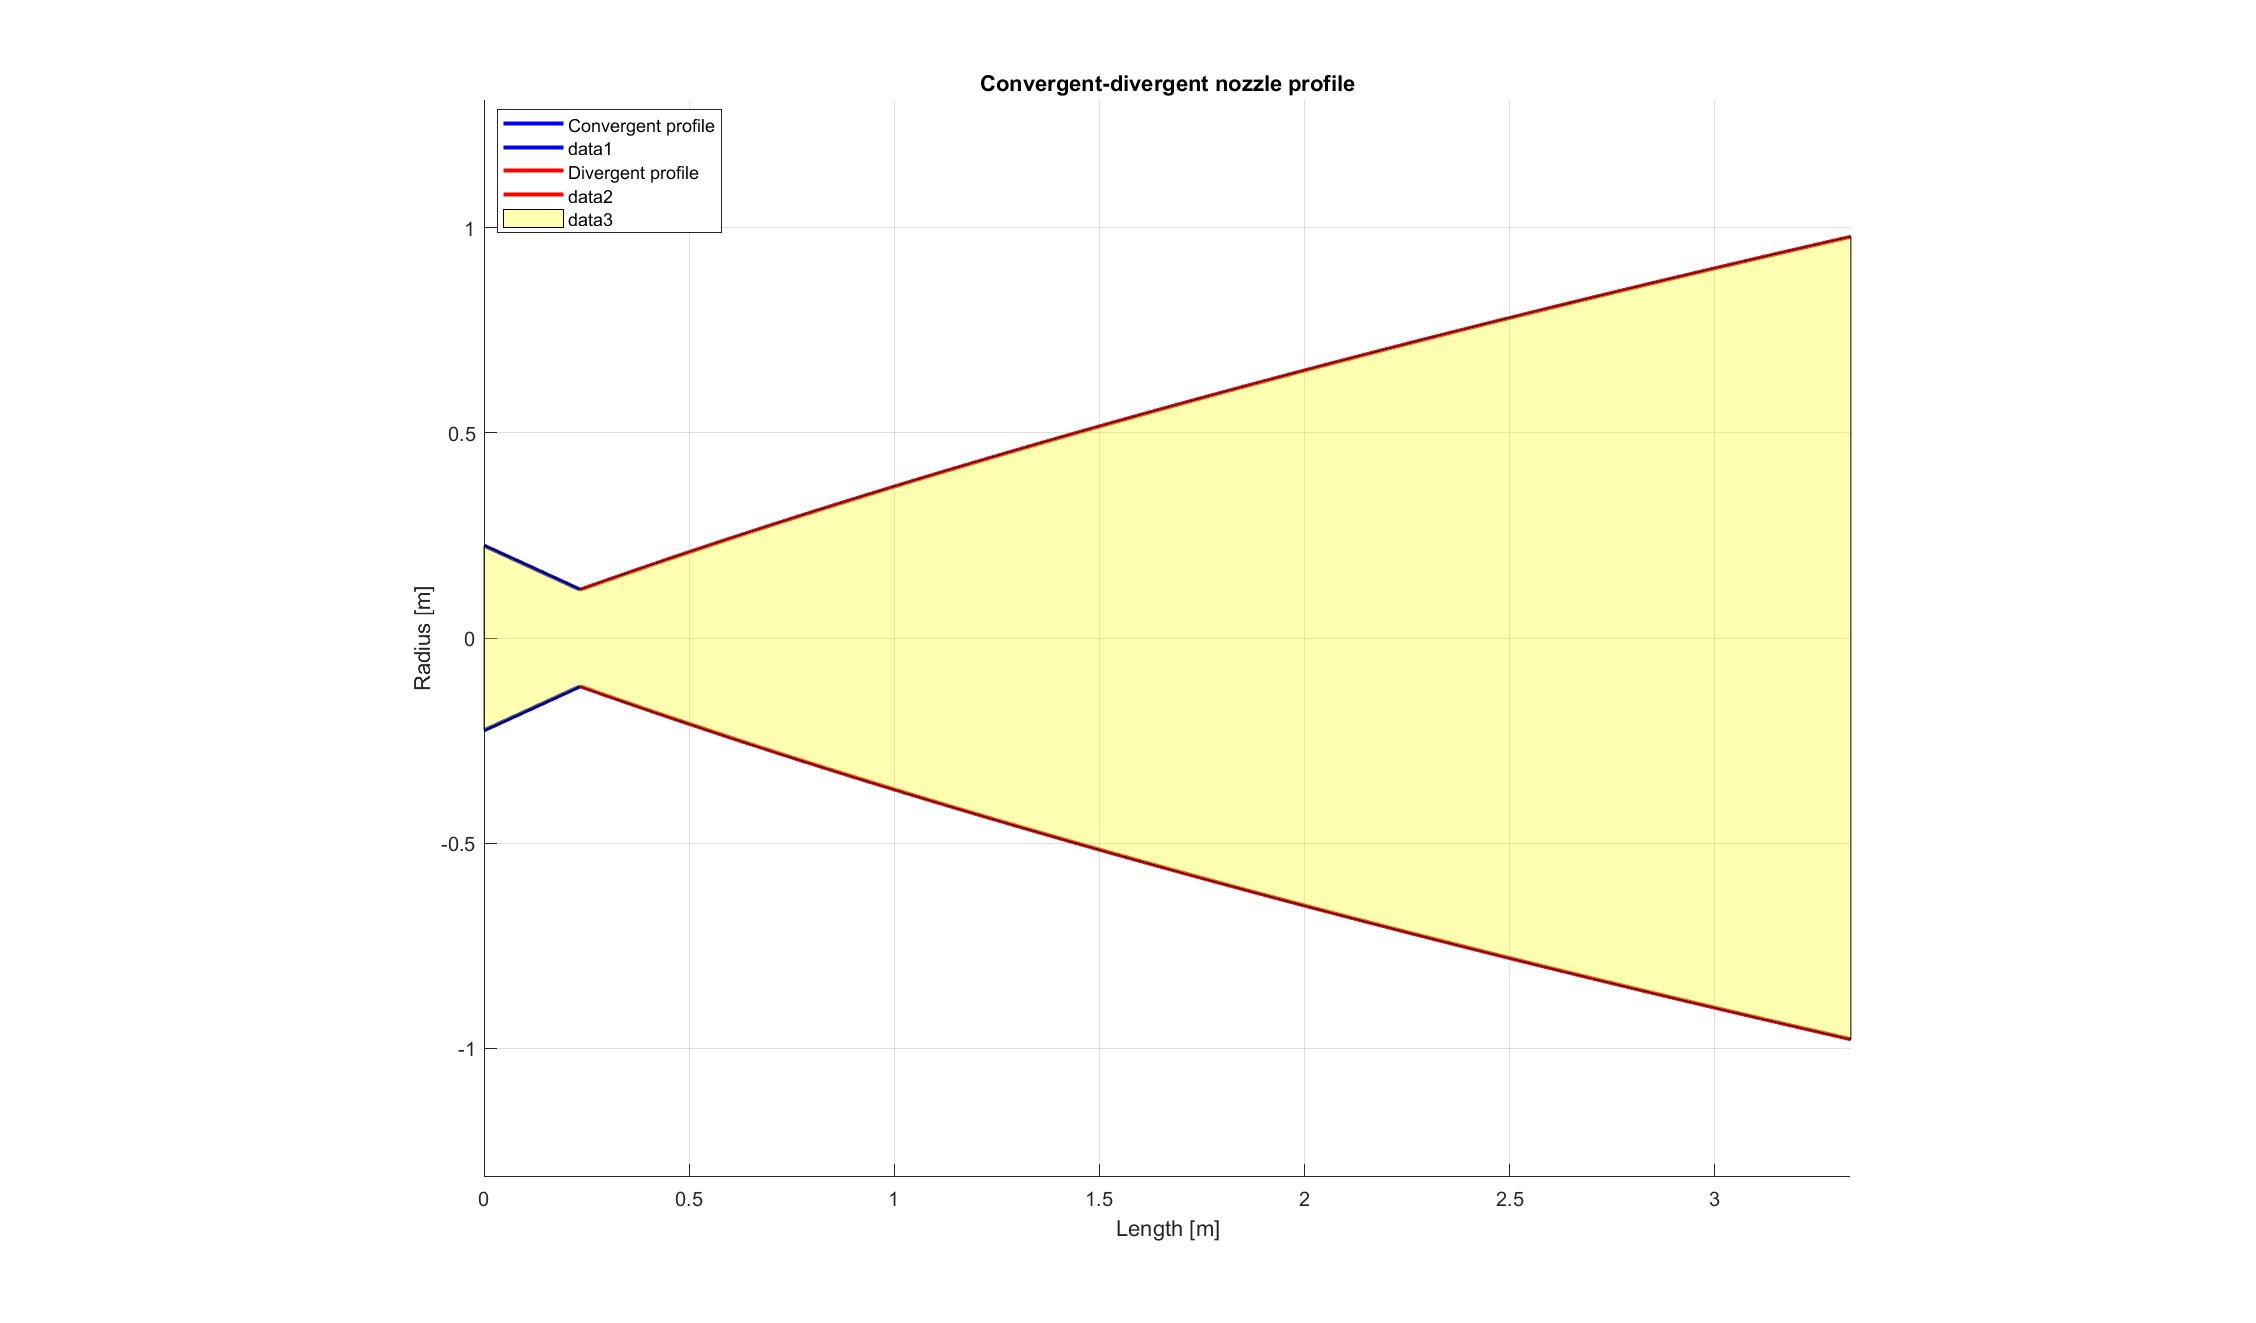
\includegraphics[width=.9\textwidth]{metao_nozzle}
	\caption{Nozzle 2D profile, case LOX/LCH4}
	\label{fig:metao_nozzle}
\end{figure}
}{.18}{.80}
\section{Conclusions}

\clearpage
\section*{Appendix A: Data utilized}
\subsection*{Classic RS-25}
\subsubsection*{Turbopumps}
\begin{table}[H]
    \centering
    \begin{tabular}{c|c}
         & \textbf{LPFTP} & \textbf{HPFTP}  & \textbf{LPOTP} & \textbf{HPOTP}\\
         $P_{in}$ [MPa] & 0.2 & 1.723 &  0.69 & 2.62\\
         $P_{out}$ [MPa] & 1.98 & 41.7 & 2.875 & 27.88\\
         $T_{in}$ [K] & 20.27 & 23.19 & 90.37 & 93\\
         $m$
    \end{tabular}
    \caption{Caption}
    \label{tab:my_label}
\end{table}
\subsubsection*{Preburners injectors design}
\subsubsection*{Performances}
\subsubsection*{External Tank design}
\begin{table}[H]
    \centering
    \begin{tabular}{|c|c|}\hline
    \textbf{Parameter} & \textbf{Value} \\ \hline
    $T$ [N] & 1860  \\\hline
    $t_b$ [s] & 480\\\hline
    $I_{sp_{sl}}$ [s] & 366\\\hline
    $O/F_{(lox/lh_2)}$ [-] & 6.03\\\hline
    \end{tabular}
    \caption{General values}
    \label{tab:tank_gen_val}
\end{table}
\begin{table}[H]
    \centering
    \begin{tabular}{|c|c|c|}\hline
    \textbf{Parameter} & \textbf{Hydrogen} & \textbf{Oxygen} \\ \hline
    $T$ [K] & 20.3 & 90.19\\ \hline
    $\rho$ [$\frac{Kg}{m^3}$]& 71.0907& 1142.4\\ \hline
    $P$ [MPa] & 0.225 & 0.680\\ \hline
    $\gamma$ [-] & 1.7097& 1.8262\\ \hline
    $M_m$ [$\frac{Kg}{Kmol}$] & 2.0157& 32\\ \hline
\end{tabular}
    \caption{Data for \acrshort{lh2} and \acrshort{lox} tanks (at tank pressure and temperature if the value is dependent by it)}
    \label{tab:data_tank_lh2_lox}
\end{table}
\begin{table}[H]
    \centering
    \begin{tabular}{|c|c|c|}\hline
        \textbf{Parameter} & \textbf{Hydrogen} & \textbf{Oxygen} \\ \hline
    $T_{\text{press}} $  [K] & 255.3722 & 448.7056 \\ \hline
    $P_{\text{press}}$ [MPa] & 21.849 & 24.607 \\ \hline
    $\gamma_{\text{press}}$ [-] & 18.0059 & 1.5102\\ \hline
\end{tabular}
    \caption{\acrshort{lch4} and \acrshort{lox} thermodynamics coordinates and values dependent by them before pressurizing the tank}
    \label{tab:data_press_lh2_lox}
\end{table}
\subsubsection*{Tank material Properties (Al 2219-T8)}
\begin{table}[H]
    \centering
    \begin{tabular}{|c|c|c|}\hline
    \textbf{Parameter} & \textbf{Value} \\ \hline
    $F_{\text{all}}$ [GPa]& 170 \\ \hline
    $\rho$ [$\frac{Kg}{m^3}$]& 2600\\ \hline
\end{tabular}
    \caption{Data relative to Al 2219-T8}
    \label{tab:data_Al2219-T8}
\end{table}
\subsubsection*{Nozzle design and profile generation}
\subsection*{Modified RS-25}
\subsubsection*{Turbopumps design}
\subsubsection*{Preburners injectors design}

\subsubsection*{Performances}

\subsubsection*{External Tank design}
\begin{table}[H]
    \centering
    \begin{tabular}{|c|c|c|}\hline
      \textbf{Parameter} & \textbf{Methane} & \textbf{Oxygen} \\ \hline
    $T$ [K] & 100 & 90.19\\ \hline
    $\rho$ [$\frac{Kg}{m^3}$]& 439.01&1142.4\\ \hline
    $P$ [MPa] & .680 & .680\\ \hline
    $\gamma$ [-] & 1.6177& 1.8262\\ \hline
    $M_m$ [$\frac{Kg}{Kmol}$] & 16.04& 32\\ \hline
\end{tabular}
    \caption{Data for \acrshort{lch4} and \acrshort{lox} tanks (at tank pressure and temperature if the value is dependent by it)}
    \label{tab:data_tank_ch4}
\end{table}

\begin{table}[H]      
    \centering
    \begin{tabular}{|c|c|c|}
    \hline
    \textbf{Parameter} & \textbf{Methane} & \textbf{Oxygen} \\ \hline
    $T_{\text{press}} $  [K] & 448.7056 & 448.7056 \\ \hline
    $P_{\text{press}}$ [MPa] & 24.6070 & 24.6070\\ \hline
    $\gamma_{\text{press}}$ [-] & 1.4001 & 1.5102\\ \hline
\end{tabular}
    \caption{\acrshort{lch4} thermodynamics coordinates and values dependent by them before pressurizing the tank}
    \label{tab:data_press_ch4}
\end{table}

For data regarding the material properties of Al 2219, refer to \cref{tab:data_Al2219-T8}.
\subsubsection*{Nozzle design and profile generation}


\printbibliography

 \end{document}
%%% TeX-master: t